\documentclass[11pt,a4paper]{article}

% ======================= PAQUETES =======================
\usepackage[utf8]{inputenc}
\usepackage[T1]{fontenc}
\usepackage[spanish]{babel}
\usepackage{graphicx}
\usepackage{geometry}
\geometry{margin=2.5cm}
\usepackage{booktabs}
\usepackage{longtable}
\usepackage{array}
\usepackage{tabularx}
\usepackage{enumitem}
\usepackage{fancyhdr}
\usepackage{titlesec}
\usepackage{xcolor}
\usepackage{hyperref}
\usepackage{caption}
\usepackage{amsmath}
\usepackage{float}
\usepackage{ragged2e}
\definecolor{titleblue}{RGB}{31,73,125}

\hypersetup{
    colorlinks=true,
    linkcolor=black,
    urlcolor=blue,
    citecolor=black,
    pdftitle={SAD: Gamma Lab},
    pdfauthor={Equipo Gamma Lab}
}

% ======================= ENCABEZADOS =======================
\pagestyle{fancy}
\fancyhf{}
\fancyhead[R]{\textbf{SAD: GAMMA LAB}}
\renewcommand{\headrulewidth}{0.4pt}
\fancyfoot[C]{\textbf{P\'agina \thepage}}
\renewcommand{\footrulewidth}{0.4pt}

\setlength{\parindent}{0pt}
\setlength{\parskip}{6pt}

% ======================= DOCUMENTO =======================
\begin{document}

% ---------------------- PORTADA ----------------------
\begin{titlepage}
\thispagestyle{empty}
\begin{center}
    % Logos institucionales (reemplazar con los archivos reales)
   %  \includegraphics[height=2cm]{logo_javeriana.png}\hspace{1cm}
    % \includegraphics[height=2cm]{logo_gammalab.png} 

    \vspace{0.5cm}
    {\large \textbf{Pontificia Universidad Javeriana}}\\
    {\large Facultad de Ingenier\'ia --- Ingenier\'ia de Sistemas}

    \vspace{1.5cm}
    {\Large\bfseries\color{titleblue} Software Architecture Document}\\
    {\large\bfseries SAD}

    \vspace{1cm}
    {\Huge\bfseries GammaLab v2.0}

    \vspace{2cm}

    \begin{tabular}{@{}ll@{}}
        \textbf{Proyecto} & Plataforma de an\'alisis y visualizaci\'on de se\~nales neurofisiol\'ogicas Gamma Lab \\
        \textbf{Documento} & Software Architecture Document --- SAD \\
        \textbf{Versi\'on} & 1.0 \\
        \textbf{Estado} & En elaboraci\'on \\
        \textbf{Fecha} & 27 de agosto de 2026 \\
    \end{tabular}

    \vspace{2cm}
    {\bfseries Autores}\\[0.3cm]
    Juan Felipe Romero Ortiz --- \texttt{juanromeroo@javeriana.edu.co}\\
    Laura Juliana Garz\'on Arias --- \texttt{garzonlj@javeriana.edu.co}\\
    Xiomara Herrera Su\'arez --- \texttt{x\_herrera@javeriana.edu.co}\\
    Sebasti\'an Almanza Galvis --- \texttt{s.almanzag@javeriana.edu.co}

\end{center}

\vfill

\noindent\textbf{Nota de uso.} Documento acad\'emico/interno del equipo de proyecto. No distribuir sin autorizaci\'on.\\
\noindent\textbf{Trazabilidad.} Este SAD define la arquitectura del sistema y traza su relaci\'on con el SRS de GammaLab v2.0.

\end{titlepage}

% ---------------------- TABLA DE CONTENIDO ----------------------
\tableofcontents
\newpage

\listoffigures
\newpage

\listoftables
\newpage

% ======================================================================
\section{Introducci\'on}

\subsection{Prop\'osito}
El presente documento describe la arquitectura de referencia del sistema GammaLab 2.0 y establece los principios, decisiones y lineamientos que orientan su diseño arquitectónico evolutivo. Expone las diferentes vistas arquitectónicas bajo el modelo 4+1 y la representación de contexto del modelo C4, proporcionando una comprensión integral de la estructura modular, los componentes y sus integraciones dinámicas. Buscar servir como un contrato técnico entre los equipos de desarrollo, validación y demás stakeholders,  garantizando una base común para la toma de decisiones, la mitigación de errores y la futura evolución del sistema. Sin contar que define los criterios necesarios para asegurar que los atributos de calidad sean evaluados y cumplirse de manera medible.

\subsection{Alcance}
Este documento abarca la definición de los principios y decisiones arquitectónicas que rigen la estructura de GammaLab v2.0, destacando el desacoplamiento de su interfaz de usuario mediante un kernel asíncrono y su extendibilidad mediante plugins. Asimismo, desarrolla las vistas lógicas, físicas, de desarrollo y de procesos del sistema, e identifica las estrategias de mitigación para riesgos críticos como el control de concurrencia en Python y el consumo acumulativo de memoria RAM. Finalmente, se definen los escenarios de calidad para la validación del sistema y su trazabilidad detallada con la especificación del SRS v2.0. Por fuera del alcance de este documento quedan las políticas de gobernanza del repositorio público de código abierto, el despliegue automatizado en entornos de integración continua (CI/CD) y las guías detalladas para el usuario final, las cuales se consolidan en el Manual de Usuario.

\subsection{Definiciones y acr\'onimos}

\begin{longtable}{@{}p{3.2cm}p{11cm}@{}}
\caption{Acr\'onimos y t\'erminos utilizados en el documento} \\
\toprule
\textbf{Sigla / T\'ermino} & \textbf{Definici\'on} \\
\midrule
\endfirsthead
\toprule
\textbf{Sigla / T\'ermino} & \textbf{Definici\'on} \\
\midrule
\endhead
SAD & Software Architecture Document. Documento de arquitectura del sistema. \\
SRS & Software Requirements Specification. Documento de especificaci\'on de requisitos. \\
SDD & Software Design Document. Documento de dise\~no t\'ecnico. \\
IoC & Inversi\'on de Control. Principio que delega el flujo de ejecuci\'on a un contenedor. \\
DI & Dependency Injection. T\'ecnica para resolver dependencias desde un contenedor externo. \\
MVP / MVC & Patrones de separaci\'on de interfaz y l\'ogica (Model--View--Presenter / Model--View--Controller). \\
Template Method & Patr\'on que define un flujo general con pasos sobrescribibles. \\
Adapter & Patr\'on para estandarizar interfaces incompatibles. \\
Caching & Estrategia para evitar recalcular o recomponer estructuras de datos. \\
Python & Lenguaje de programaci\'on principal de \textit{Gamma Lab}. \\
PyQt5 & Framework de interfaz gr\'afica basado en Qt para Python. \\
VTK & Visualization Toolkit. Biblioteca para visualizaci\'on cient\'ifica 2D/3D. \\
QVTK & Interfaz \texttt{QVTKRenderWindowInteractor} para incrustar VTK en aplicaciones Qt. \\
NumPy & Librer\'ia para c\'alculo num\'erico vectorizado. \\
EDF & European Data Format. Formato est\'andar para se\~nales biom\'edicas. \\
ABF & Axon Binary File. Formato de archivo utilizado por Axon Instruments para registros biom\'edicos. \\
GUI Toolkit & Conjunto de herramientas para construir interfaces gr\'aficas (Qt, PyQt, VTK). \\
\bottomrule
\end{longtable}

\subsection{Audiencia}
Este documento está dirigido al equipo de desarrollo, así como a cualquier stakeholder con formación técnica que requiera comprender las decisiones arquitectónicas del sistema. Asimismo, está orientado a todos los investigadores y personas del Laboratorio de Electrofisiología de la Universidad de Colombia que estén interesados en conocer la estructura interna, los principios de diseño y los mecanismos de GammaLab v2.0 para el uso, mantenimiento y futuros cambios.

\subsection{Referencias relacionadas}
Este SAD se alinea con:
\begin{itemize}[nosep]
    \item \textbf{SRS de Gamma Lab}: requisitos funcionales y no funcionales del sistema.
\end{itemize}

Las referencias t\'ecnicas externas (PyQt, VTK, NumPy, EDF/ABF, YAML).

% ======================================================================
\section{Contexto del sistema}

\subsection{Visi\'on general}
GammaLab v2.0 está estructurado como una aplicación de escritorio tipo standalone diseñada para ser ejecutada de forma local, sin requerir conectividad de red. Su arquitectura se basa en un patrón modular de microkernel, donde un núcleo central asíncrono (desarrollado en Python con el framework gráfico PySide6 y la librería de visualización científica VTK) orquesta la ejecución y comunicación de plugins independientes a través de un almacén de datos en memoria (DataStore). 
La evolución fundamental de esta segunda iteración se muestra una evolución de los hilos únicos de Python, mediante la incorporación de estrategias de paralelización basadas en multiprocesamiento y multithreading en el kernel. Esto permite que el sistema distribuya las tareas pesadas (como la transformada Wavelet y el acoplamiento cruzado de frecuencias) sin congelar la interfaz de usuario.

\subsection{L\'imites del sistema}

\subsubsection{Dentro del alcance}
\begin{itemize}[nosep]
    \item \textbf{Ingreso y lectura:} Carga nativa de registros electroencefalográficos (EEG) almacenados localmente en formatos estándares .edf, .abf, .bdf y .mat.
    \item \textbf{Procesamiento y segmentación:} Aplicación de filtros digitales de corte, remoción de artefactos de estimulación y segmentación de señales en ensayos (trials) mediante umbrales en mV u operaciones de intervalo interestímulo (ISI).
    \item \textbf{Procesamiento espectral y tiempo-frecuencia:} Cálculo de promedios de Potenciales Relacionados a Eventos (ERP) con visualización de Butterfly plot bajo demanda, análisis de Transformada Rápida de Fourier (FFT), Densidad Espectral de Potencia (PSD) y Transformada Wavelet Continua con normalización y escalas personalizables.
    \item \textbf{Análisis de conectividad y acoplamiento avanzado:} Ejecución del análisis de acoplamiento fase-amplitud (PAC) tanto de un canal como cruzado intercanal.
    \item \textbf{Persistencia del espacio de trabajo:} Guardado y restauración del estado de la sesión analítica mediante archivos de proyecto local con extensión personalizada .glab.
    \item \textbf{Exportación de resultados:} Generación de archivos de datos numéricos estructurados (CSV con ejes X simplificados, Excel, JSON) y representaciones gráficas de alta resolución, incluyendo formato de imagen estándar (PNG, JPG, TIFF) e imagen vectorial científica (EMF).
\end{itemize}

\subsubsection{Fuera del alcance}
\begin{itemize}[nosep]
    \item La comunicación o adquisición de señales EEG en tiempo real mediante conexiones directas a equipos de amplificación, electrodos o diademas inalámbricas.
    \item La persistencia de proyectos en bases de datos centralizadas, servicios en la nube, servidores remotos o API web distribuidas; toda la persistencia es local e individual.
    \item El soporte operativo para plataformas web, sistemas móviles o sistemas operativos Unix/macOS en distribución comercial nativa (el instalador standalone se restringe a Windows de 64 bits).
    \item Mecanismos de control de acceso multiusuario, autenticación de seguridad en red, cifrado de datos clínicos o sincronización colaborativa síncrona.
\end{itemize}

\subsubsection{Entradas externas}
\begin{itemize}[nosep]
    \item  Señales neurofisiológicas digitalizadas en formatos binarios compatibles (.edf, .abf, .bdf, .mat).
    \item Configuración alfanumérica de entrada por el usuario clínico (frecuencias de muestreo, umbrales de trial en mV, bandas de frecuencia de fase/amplitud para PAC/PLV y ciclos de wavelet).
    \item Eventos de interacción directa del investigador con la GUI mediante teclado y ratón para realizar zoom multidireccional, desplazamiento temporal (pan) y selección de puntos específicos sobre las gráficas para la toma de medidas.
\end{itemize}

\subsubsection{Salidas externas}
\begin{itemize}[nosep]
    \item Gráficas 2D renderizadas mediante VTK embebido en PySide6, tales como comodulogramas de PAC, mapas de calor de coherencia temporal-frecuencial y espectrogramas Wavelet.
    \item Archivos con metadatos y estados serializados .glab que contienen los análisis intermedios, rutas absolutas y configuraciones del proyecto.
    \item Tablas de resultados analíticos en formato Excel (.xlsx), JSON y archivos CSV optimizados para evitar redundancia de ejes temporales.
    \item Archivos de imagen estándar (PNG/JPG/TIFF) y gráficos vectoriales de alta precisión (EMF) para uso directo en publicaciones indexadas.
\end{itemize}

% ======================================================================
\section{Metas y Restricciones de la Arquitectura}

\subsection{Requisitos de los Stakeholders}

\begin{longtable}{@{}>{\raggedright\arraybackslash}p{3.2cm}
                  >{\raggedright\arraybackslash}p{2.5cm}
                  >{\raggedright\arraybackslash}p{8.8cm}@{}}

\caption{Stakeholders principales y expectativas} \\
\toprule

\textbf{Stakeholder} &
\textbf{Tipo} &
\textbf{Necesidades / Intereses} \\

\midrule
\endfirsthead

\toprule
\textbf{Stakeholder} &
\textbf{Tipo} &
\textbf{Necesidades / Intereses} \\
\midrule
\endhead

Laboratorio de Electrofisiología de la Universidad de Colombia
&
Usuario final
&
Su interés principal es contar con una herramienta robusta, intuitiva y libre de licencias que simplifique el análisis complejo por medio de PAC, sin necesitar habilidades de programación.
\\[0.3cm]

Equipo de desarrollo
&
Interno
&
Implementar una arquitectura extensible (microkernel + plugins), reestructurar el diseño de las pantallas aplicando estándares de codificación limpia y utilizar paralelización asíncrona.
\\[0.3cm]

Directora de tesis
&
Interno
&
Validar la rigurosidad científica de los algoritmos de frecuencia y supervisar el cumplimiento del alcance metodológico.
\\[0.3cm]

Evaluadores académicos
&
Externo / Validador
&
Verificar el cumplimiento de requerimientos, funciones y metodología aplicada desde la ingeniería de sistemas e ingeniería electrónica, demostrando cuantitativamente la mejora de rendimiento con respecto a GammaLab v1.0.
\\[0.3cm]

Comunidad científica
&
Externo / Colaborador
&
Posibilidad de reutilizar y mejorar el código abierto; transparencia metodológica y reproducibilidad de resultados; estandarización de flujos de trabajo y formatos de análisis EEG.
\\

\bottomrule

\end{longtable}

\subsection{Atributos de Calidad}

\label{sec:atributos_calidad}

La arquitectura de \textbf{GammaLab 2.0} fue diseñada pensando principalmente en las necesidades manifestadas en el laboratorio de electrofisiología, entendiendo sus flujos de trabajo y los requerimientos propios de la ejecución de análisis experimentales. Al mismo tiempo, 
se proyecta como un software adaptable a distintos contextos y paradigmas de investigación, por lo que resulta fundamental considerar el impacto de los siguientes atributos de calidad en esta segunda versión:

\begin{enumerate}
    \item \textbf{Extensibilidad:} Dado que el sistema debe adaptarse tanto a diferentes tipos de experimentos como a diversos entornos de investigación, la extensibilidad se concibe como una capacidad primordial. El diseño permite agregar nuevos módulos personalizados, 
    completamente programables por cada laboratorio o usuario, y ofrece una interfaz clara para integrarlos de manera sencilla dentro del sistema. En \textbf{GammaLab 2.0}, esta capacidad se optimiza al desacoplar los plugins del núcleo mediante un contenedor de
     \textbf{Inversión de Control (IoC)}, registrando servicios comunes (como \texttt{ExportService}, \texttt{MeasurementService} y \texttt{SettingsService}) que evitan importaciones directas o acoplamientos rígidos. Asimismo, la entidad \texttt{SignalDataset} expone una 
     API pública de comunicación estricta que encapsula la manipulación de trials, garantizando que futuras extensiones no alteren la integridad de los datos en memoria.
    
    \item \textbf{Usabilidad:} GammaLab se privilegia de un diseño de interfaz de usuario pensado para ser lo más sencillo y entendible posible en cada funcionalidad implementada. Lo anterior resulta especialmente importante en el caso de los plugins, donde se manejan procesos 
    conceptualmente complejos. En esta nueva versión, se eliminan las barreras técnicas de uso mediante ayudas contextuales integradas (\textit{tooltips}) para todos los parámetros, menús unificados de edición en la vista principal (\textit{Home}) y la representación 
    explícita de gráficas complejas como el \textit{Butterfly plot}. Adicionalmente, el sistema asegura la retroalimentación constante del estado del sistema mediante barras de progreso no bloqueantes para operaciones superiores a 1 segundo, garantizando un flujo intuitivo y controlado.
    
    \item \textbf{Mantenibilidad:} La arquitectura propuesta favorece la modularidad y el ordenamiento claro del código, buscando que el sistema siga principios como el de Abierto/Cerrado dentro del marco SOLID: abierto a extensiones y cerrado a modificaciones innecesarias. El sistema realiza una separación
     rigurosa entre la interfaz gráfica (PySide6) y la lógica matemática en hilos de cómputo independientes, facilitando la depuración del código. Además, la mantenibilidad y la robustez técnica se garantizan mediante el apego estricto a las directrices de estilo \textbf{PEP8} y un estándar mínimo del 
     \textbf{80\% de cobertura de pruebas unitarias automatizadas} utilizando el framework \textbf{Pytest}.
    
    \item \textbf{Rendimiento:} El contexto de uso del programa exige un rendimiento estable y un consumo controlado de recursos, especialmente dada la naturaleza de los datos involucrados, que suelen tener alta densidad de información. Para dar soporte estable a señales de hasta 600~MB en memoria, \textbf{GammaLab 2.0} 
    incorpora una estrategia de paralelización en el Kernel. Las tareas pesadas de procesamiento (PAC, Wavelet, PSD) se distribuyen de forma asíncrona mediante multiprocesamiento (\texttt{multiprocessing}), impidiendo que la interfaz gráfica se bloquee durante los análisis (manteniendo la responsividad $\le$ 0.3~s). Adicionalmente, 
    se introduce el submuestreo dinámico visual a un límite de 2000 puntos por serie en los widgets de VTK para conservar una navegación fluida ($\ge$ 24~FPS) sin degradar la data cruda, acompañado de rutinas explícitas de liberación de memoria de GPU y RAM en cada plugin al cambiar de módulo.
    
    \item \textbf{Portabilidad:} El sistema debe asegurar su correcta ejecución en diversos entornos locales sin requerir la intervención técnica continua del equipo desarrollador. \textbf{GammaLab 2.0} centraliza su portabilidad local en sistemas Windows 10/11 de 64 bits. Este atributo se consolida al empaquetar la aplicación de manera autónoma
     en un \textbf{ejecutable standalone (.exe)} a través de PyInstaller. Esto permite que el personal clínico e investigadores ejecuten análisis avanzados localmente con un doble clic, omitiendo por completo la configuración o instalación manual de librerías científicas y consolas de Python en sus estaciones de trabajo.
    
    \item \textbf{Robustez y Fiabilidad:} El sistema debe mantener la estabilidad operativa en sesiones continuas y tolerar errores imprevistos en tiempo de ejecución. Ante excepciones internas generadas por plugins de terceros o formatos de archivo corruptos, el sistema captura los fallos de manera centralizada sin interrumpir la sesión del usuario ni provocar la
     caída de la aplicación. Adicionalmente, el sistema implementa exclusiones mutuas para accesos concurrentes al almacén de datos centralizado (\textit{DataStore}), asegura la correcta liberación de observadores y callbacks VTK y proporciona terminaciones controladas (\textit{cleanup}) de hilos de procesamiento de datos ante solicitudes explícitas de cancelación.
    
    \item \textbf{Trazabilidad y Persistencia:} El sistema incorpora en cada análisis la información contextual y los metadatos necesarios para asegurar la reproducibilidad y trazabilidad de los resultados. \textbf{GammaLab 2.0} materializa esta capacidad de forma completa mediante el módulo \textbf{PJ (Project Session)}, el cual introduce la persistencia local 
    del estado completo del espacio de trabajo (rutas de señales, trials configurados y análisis procesados) en archivos con extensión de proyecto \textbf{.glab} o \textbf{.glws}. Asimismo, la trazabilidad científica externa se respalda al exportar resultados consistentes en formatos tabulares (CSV sin redundancia de ejes temporales, Excel, JSON) 
    y gráficos de alta calidad vectorial en formato \textbf{EMF}.
\end{enumerate}


\begin{enumerate}
    \item 
\end{enumerate}

\subsection{Supuestos y limitaciones derivadas}
A continuaci\'on se presentan los supuestos y limitaciones considerados durante el dise\~no y construcci\'on del sistema:

\subsubsection{Restricciones de arquitectura}
    \begin{itemize}
        \item \textbf{Operación standalone y offline:} El sistema debe ejecutarse de forma local en la máquina del investigador de forma estricta. No se permite el uso de servicios en la nube, APIs de procesamiento externas ni el uso de bases de datos distribuidas.
        \item \textbf{Entorno tecnológico base:} El núcleo matemático y la lógica de interacción deben desarrollarse bajo el lenguaje Python (versión mínima 3.11), utilizando Pyside6 para la interfaz y VTK para la visualización científica.
        \item \textbf{Compatibilidad de datos:} El módulo de entrada/salida soporta y procesa archivos de señales en formatos como: EDF, ABF, BDF, MAT y GLAB.
    \end{itemize}   

\subsubsection{Supuestos de operación (Evolución de v1.0)}
    \begin{itemize}
        \item \textbf{Procesamiento concurrente:} En esta nueva versión 2.0 se asume que el hardware cuenta con arquitectura multinúcleo (más de 4 núcleos) para el despliegue de procesamiento asíncrono y multiprocesamiento en segundo plano.
        \item \textbf{Naturaleza del proyecto:} El sistema está diseñado exclusivamente para el posprocesamiento y análisis de señales previamente adquiridas. No soporta adquisición de datos en tiempo real ni comunicación con hardware de amplificación o registro fisiológico.
    \end{itemize}

% ======================================================================
\section{Principios y decisiones arquitect\'onicas}

\subsection{Estilo base}

La arquitectura de GammaLab 2.0 adopta un estilo microkernel, en el que el sistema central o \textit{core system} proporciona los servicios esenciales de comunicación, gestión de plugins, registro de eventos, coordinación de tareas y manejo de datos. Este núcleo actúa como mediador entre los distintos módulos funcionales del sistema, permitiendo que cada plugin se conecte e interactúe mediante una interfaz común, sin acoplarse directamente a la lógica interna del sistema.

El \textit{Kernel} es el componente central de esta arquitectura y desempeña la función de orquestador principal. Su responsabilidad consiste en coordinar la ejecución de tareas, gestionar la cola de trabajos, supervisar el estado de cada operación, controlar la cancelación de procesos en ejecución y administrar la sincronización entre la interfaz gráfica y los módulos de análisis. De esta forma, la capa de presentación permanece responsiva mientras el procesamiento de señales y cálculos estadísticos se ejecutan en segundo plano.

La separación entre la lógica estable del sistema y la funcionalidad específica de análisis es una de las decisiones más relevantes del diseño. El \textit{core} encapsula los servicios transversales de la aplicación, como el almacenamiento de datos, la gestión de eventos, la carga de archivos, la exportación de resultados y la configuración del entorno operativo. Por su parte, los plugins especializados implementan las distintas capacidades del sistema, como FFT, PSD, Wavelet, ERP, PAC y otras herramientas de análisis.

Esta estructura favorece la extensibilidad del sistema, ya que permite incorporar nuevos módulos funcionales sin modificar la lógica del núcleo. Además, reduce el acoplamiento entre componentes y mejora la mantenibilidad del proyecto a lo largo de su evolución. La relación entre el \textit{core} y los plugins se establece a través de una API de integración basada en la interfaz \textit{IPlugin}, la cual define el contrato que cada módulo debe cumplir para incorporarse al ecosistema de GammaLab 2.0.

En este sentido, la arquitectura del sistema se organiza en tres capas principales: la capa de presentación, donde se encuentra la interfaz gráfica desarrollada con PySide6 y Qt; la capa de coordinación, representada por el Kernel y los servicios compartidos del core; y la capa funcional, conformada por los plugins que implementan los distintos análisis y visualizaciones.
\begin{figure}
    \centering
    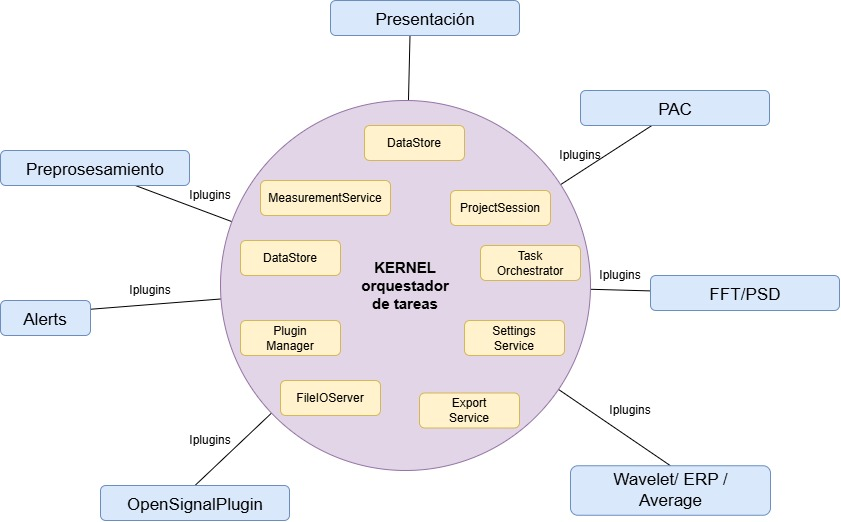
\includegraphics[width=0.95\linewidth]{DiagramaEstiloBase.jpg}
    \caption{Diagrama conceptual de la arquitectura microkernel de GammaLab 2.0, mostrando la relación entre el núcleo central, los servicios compartidos y los plugins especializados.}
    \label{fig:estilo_base_microkernel}
\end{figure}

\subsubsection{Orquestador del sistema}

El Kernel de GammaLab 2.0 se define como el orquestador central del sistema. Su principal función es coordinar la ejecución de tareas complejas y garantizar que las operaciones intensivas de cómputo no bloqueen la interfaz gráfica. Esta decisión es clave para el rendimiento del sistema, ya que el análisis de señales EEG implica el manejo de datos de alta resolución, filtros, transformadas, estimaciones de potencia y análisis de acoplamiento cruzado de frecuencias.

Entre las funciones del orquestador se encuentran:

\begin{itemize}
    \item Registro y descubrimiento de plugins.
    \item Gestión de la cola de tareas y priorización de ejecución.
    \item Distribución de tareas entre hilos o procesos según su complejidad.
    \item Control del estado de cada operación: pendiente, ejecutándose, completada o cancelada.
    \item Supervisión del progreso de los análisis.
    \item Coordinación con los servicios del core.
    \item Entrega de resultados hacia la capa visual.
    \item Gestión de errores y alertas a la interfaz de usuario.
\end{itemize}

El orquestador actúa como el punto de integración entre la capa de presentación, los servicios del sistema y los módulos especializados. Cuando el usuario solicita ejecutar un análisis, la interfaz no invoca directamente la lógica del plugin; en cambio, la solicitud se envía al Kernel, quien valida el contexto, identifica el módulo apropiado, crea la tarea y la ejecuta de forma controlada. Esta estructura evita duplicación de lógica, reduce fallos de sincronización y mejora la trazabilidad de las operaciones.

En términos arquitectónicos, el Kernel también centraliza la administración de recursos del sistema. Esto incluye la gestión de la memoria compartida, la preparación de datos para análisis y la actualización del estado global del entorno. En un sistema orientado a señales neurofisiológicas, donde los volúmenes de información pueden ser elevados, esta coordinación es crítica para asegurar estabilidad, eficiencia y capacidad de respuesta.

\subsubsection{Componentes del núcleo}

El núcleo de GammaLab 2.0 está conformado por una serie de componentes que permiten la operación global del sistema. Estos módulos no son reemplazables por plugins, sino que constituyen la base funcional sobre la cual todo el entorno opera.

Los principales componentes del core son:

\begin{itemize}
    \item \textbf{Kernel}: responsable de la orquestación y coordinación de tareas.
    \item \textbf{PluginManager}: encargado de registrar, validar y cargar los plugins disponibles.
    \item \textbf{DataStore}: almacena señales, resultados intermedios, metadatos, configuraciones y sesión activa.
    \item \textbf{FileIOService}: gestiona la lectura y validación de archivos EEG en formatos como ABF, EDF, BDF y MAT.
    \item \textbf{MeasurementService}: administra métricas, cálculos y resultados derivados del análisis.
    \item \textbf{SettingsService}: maneja la configuración general del sistema y preferencias del usuario.
    \item \textbf{ExportService}: se encarga de la exportación de resultados en formatos compatibles con análisis e informes.
    \item \textbf{ProjectSession}: gestiona la persistencia del espacio de trabajo mediante archivos de proyecto \texttt{.glab}, guardando y restaurando la señal activa, los trials, los análisis y los parámetros de la sesión.
\end{itemize}

El diseño del núcleo sigue un principio de servicio compartido, donde los plugins no crean instancias aisladas de cada funcionalidad, sino que acceden a los servicios del sistema mediante interfaces controladas por el Kernel. Este enfoque reduce el acoplamiento entre módulos y facilita la evolución del sistema sin afectar la lógica base.

\subsubsection{Arquitectura basada en plugins}

GammaLab 2.0 implementa una arquitectura modular basada en plugins, con el objetivo de ampliar la funcionalidad del sistema sin modificar el núcleo central. Cada plugin encapsula una capacidad específica de análisis o visualización, y se integra con la aplicación mediante un contrato común definido por la interfaz \textit{IPlugin}.

Un plugin de GammaLab 2.0 puede contener:

\begin{itemize}
    \item lógica de procesamiento,
    \item componentes de interfaz gráfica,
    \item configuraciones específicas del análisis,
    \item metadatos de identificación,
    \item conexión con el DataStore y el Kernel.
\end{itemize}

El \textit{PluginManager} realiza el descubrimiento dinámico de nuevos módulos, validando la presencia de metadatos y registrando cada extensión dentro del ecosistema del sistema. Esta estructura permite que el sistema evolucione de forma incremental: cada nuevo módulo puede añadirse a la aplicación sin recompilar el núcleo ni modificar la lógica general del software.



\subsubsection{Principio de desacoplamiento y extensibilidad}

La arquitectura de GammaLab 2.0 se fundamenta en el principio de desacoplamiento funcional. La capa de presentación, el Kernel y los plugins mantienen una separación clara de responsabilidades. Esta decisión permite que cada módulo evolucione de forma independiente sin comprometer la estabilidad general del sistema. Por ejemplo, una modificación en la interfaz de usuario no exige cambiar la lógica del análisis; un nuevo módulo de procesamiento puede agregarse sin alterar la estructura del núcleo; y una actualización en la gestión de archivos no afecta directamente a la visualización de resultados.

La extensibilidad también se ve reforzada por un conjunto de mecanismos bien definidos:

\begin{itemize}
    \item Registro dinámico de plugins.
    \item Contrato de integración mediante IPlugin.
    \item Gestión centralizada de datos mediante DataStore.
    \item Coordinación de tareas mediante el Kernel.
    \item Desacoplamiento entre lógica funcional y visualización.
\end{itemize}


\subsubsection{Justificación}

La arquitectura adoptada para GammaLab 2.0 corresponde a un estilo microkernel, en el que el núcleo central del sistema es el core y, dentro de este, el Kernel cumple la función de orquestador principal. Esta decisión permite separar la lógica estable del sistema de las funcionalidades específicas de análisis, manteniendo un diseño modular, extensible y de bajo acoplamiento.

El Kernel centraliza la coordinación de tareas, la gestión de la cola de ejecución, la supervisión del estado de cada operación y la delegación de la lógica funcional a los plugins. Esta decisión es necesaria porque el procesamiento de señales EEG requiere operaciones computacionalmente intensivas, como PAC, FFT, PSD y Wavelet, que no deben ejecutarse directamente en la interfaz gráfica. Además, al separar la lógica de coordinación del procesamiento funcional, el sistema mantiene un mejor control del flujo de trabajo, facilita la gestión de errores y cancelaciones, y permite una ejecución más ordenada de tareas en segundo plano. Esto mejora la experiencia del usuario, reduce la carga operativa del sistema y favorece la extensibilidad del proyecto, ya que nuevos plugins pueden añadirse sin afectar el funcionamiento del núcleo ni la interfaz.

Esta organización facilita la incorporación de nuevos módulos sin modificar el núcleo, reduce la dependencia entre componentes y permite un mejor control del flujo de datos y de los resultados. La integración con servicios compartidos como DataStore, FileIOService, MeasurementService y ExportService garantiza un manejo más ordenado de la información, la persistencia y la visualización de resultados.



\subsubsection{Decisiones arquitectónicas}

Conforme evolucionaba el proyecto, también lo hacían las decisiones arquitectónicas necesarias para alcanzar el estado final de la implementación. Los problemas, restricciones y hallazgos identificados durante el proceso guiaron la selección y el ajuste de cada componente del diseño. A continuación se listan las decisiones arquitectónicas con mayor impacto dentro del proyecto:

\begin{table}[H]
    \centering
    \caption{ADRs resumidas: decisión, motivación y consecuencias.}
    \begin{tabular}{|p{0.14\textwidth}|p{0.26\textwidth}|p{0.24\textwidth}|p{0.28\textwidth}|}
        \hline
        \textbf{ID} & \textbf{Decisión} & \textbf{Motivación} & \textbf{Consecuencias} \\
        \hline
        ADR-01 & Estilo arquitectónico de microkernel. & Permitir la incorporación de nuevas funcionalidades al sistema, incluso en tiempo de ejecución. & Sistema modular, ampliable y con bajo acoplamiento; mayor complejidad inicial. \\
        \hline
        ADR-02 & Separación entre core, plugins y app. & Organizar responsabilidades y mantener claridad modular. & Facilita la comprensión, el mantenimiento y el desarrollo incremental. \\
        \hline
        ADR-03 & Interfaz IPlugin. & Aplicar inversión de control para que los plugins definan únicamente su lógica. & Menor acoplamiento. \\
        \hline
        ADR-04 & Carga dinámica de plugins. & Permitir la incorporación de módulos sin recompilar. & Mejor extensibilidad y colaboración entre equipos. \\
        \hline
        ADR-05 & Uso de Python, PySide6 y VTK. & Utilizar librerías maduras para visualización científica y GUI. & Base sólida para análisis; requiere control cuidadoso de rendimiento y memoria. \\
        \hline
        ADR-06 & Uso de DataStore. & Evitar duplicaciones y permitir la propagación reactiva de cambios. & Coherencia global y ahorro de memoria; requiere un diseño cuidadoso. \\
        \hline
        ADR-07 & Kernel como orquestador central. & Ejecutar tareas pesadas sin bloquear la interfaz ni acoplar cada módulo al core. & Mayor control de concurrencia, cancelación, prioridad y trazabilidad. \\
        \hline
        ADR-08 & Estructura estándar del plugin. & Unificar lógica, interfaz gráfica, metadatos y configuración. & Mejor mantenibilidad y estandarización. \\
        \hline
        ADR-09 & Soporte explícito para PAC y análisis de acoplamiento. & Incorporar análisis avanzados de señales neurofisiológicas. & Mayor alcance funcional y nuevas dependencias especializadas. \\
        \hline
    \end{tabular}
\end{table}

\subsubsection{Patrones utilizados}

A continuación se presenta un resumen de los patrones arquitectónicos aplicados en el diseño de GammaLab 2.0, alineados con el estilo microkernel, el mecanismo de plugins y los servicios internos del sistema:



\begin{table}[H]
\centering
\caption{Patrones arquitectónicos aplicados en GammaLab 2.0.}
\label{tab:patrones_arquitectonicos}
\renewcommand{\arraystretch}{1.15}
\begin{tabularx}{\columnwidth}{|p{0.20\columnwidth}|p{0.27\columnwidth}|X|}
\hline
\textbf{Patrón} &
\textbf{Problema que resuelve} &
\textbf{Aplicación en GammaLab 2.0} \\
\hline

Plugin &
Agregar capacidades sin modificar el núcleo del sistema. &
Cada plugin define un archivo \texttt{properties.yaml} y una clase que implementa \texttt{IPlugin}. El Kernel los descubre dinámicamente y los vincula en tiempo de ejecución. \\
\hline

IoC / Service Locator (Kernel) &
Reducir el acoplamiento y centralizar los servicios compartidos. &
El Kernel registra y expone servicios como \textit{DataStore}, \textit{FileIOService}, \textit{ExportService}, \textit{MeasurementService} y \textit{SettingsService}. Los plugins acceden a estos servicios sin crear instancias propias. \\
\hline

Adapter (NumPy a VTK) &
Integrar estructuras científicas con componentes de visualización. &
El módulo \textit{vtk adapters} convierte arrays de NumPy en \textit{vtkTable} o estructuras compatibles para su uso en \textit{vtkChartXY} y otros componentes VTK. \\
\hline

MVP / MVC en interfaz &
Separar la vista de la lógica de interacción. &
\textit{MainWindow} gestiona la navegación y composición; cada plugin proporciona su interfaz mediante \texttt{get\_widget()}, mientras que la lógica reside en \texttt{process()}, \texttt{start()} y \texttt{stop()}. \\
\hline

Caching (datos y widgets) &
Reducir la latencia y la recomputación innecesaria. &
Se almacenan en caché datos, resultados intermedios y widgets de plugins previamente inicializados. \\
\hline

Template Method (ciclo de vida) &
Definir puntos de extensión uniformes. &
\texttt{IPlugin} establece métodos clave (\texttt{initialize}, \texttt{start}, \texttt{process}, \texttt{stop} y \texttt{get\_widget}) que todo plugin debe implementar. \\
\hline

Task orchestration / Executor pattern &
Gestionar cálculos pesados sin bloquear la interfaz. &
El Kernel centraliza la ejecución de tareas, su cola, cancelación, seguimiento del progreso y entrega de resultados. \\
\hline

\end{tabularx}
\end{table}




% ======================================================================
\section{Vistas Arquitect\'onicas (4+1)}

\subsection{Objetivo}
Concretar \textbf{escenarios} que ejerciten decisiones y atributos de calidad de Gamma Lab 2.0. A diferencia de Gamma Lab 1.0 (sistema ya construido), Gamma Lab 2.0 documenta un sistema \textbf{parcialmente existente}: cada vista distingue expl\'icitamente qu\'e componentes \textbf{ya existen} en el c\'odigo actual y cu\'ales son \textbf{nuevos}, por construir a partir de los 23 casos de uso (CU-001 a CU-023) especificados en el documento ISTAR. Cada escenario se especifica con el formato: \textit{(Est\'imulo, Fuente, Entorno, Artefacto, Respuesta, Medida de respuesta)} y se vincula con los CU y requisitos (R-XX) que lo originan.

\subsection{Vista de Escenarios}

\begin{figure}[htbp]
    \centering
    \includegraphics[width=0.95\linewidth]{diagrama_casos_de_uso_sistema_completo.png}
    \caption{Diagrama de casos de uso del sistema completo Gamma Lab 2.0 (23 CU en 5 subsistemas). Las relaciones \textit{include}/\textit{extend} se tomaron literalmente del campo ``Extensiones'' de cada ficha; ninguna es inferida por similitud tem\'atica.}
    \label{fig:vistacasosuso}
\end{figure}

La Figura \ref{fig:vistacasosuso} revela que el subsistema \textbf{N\'ucleo y Ciclo de Vida} --- en particular CU-020, el orquestador de tareas --- es el verdadero centro de gravedad arquitect\'onico: diez de los otros veintid\'os casos de uso lo incluyen expl\'icitamente. Esa centralidad se concreta a continuaci\'on en tres escenarios representativos.

\begin{table}[htbp]
\centering
\caption{UC-01 --- Calcular acoplamiento fase-amplitud (PAC) de un canal}
\begin{tabularx}{\linewidth}{@{}p{2.6cm}X@{}}
\toprule
\textbf{Est\'imulo} & El investigador configura banda de fase, rango de amplitud y trial \'unico/promedio, y pulsa ``Calcular PAC'' (CU-001). \\
\textbf{Fuente} & Usuario final (investigador). \\
\textbf{Entorno} & Existe un \texttt{TrialDataset} activo en \texttt{DataStore} (CU-004/CU-006 ya ejecutados); plugin \texttt{PACSingleChannelPlugin} activo, categor\'ia \textit{Analysis} \textbf{(nuevo)}. \\
\textbf{Artefacto} & \texttt{PACSingleChannelPlugin} \textbf{(nuevo)}, \texttt{Task\-Orchestrator} \textbf{(nuevo)}, \texttt{DataStore} (ya existe), adaptadores VTK (ya existen). \\
\textbf{Respuesta} & El plugin delega el c\'omputo de la transformada wavelet al orquestador del n\'ucleo en vez de instanciar hilos propios; al finalizar, publica el mapa fase-frecuencia, el histograma de fase y el vector de acoplamiento medio, y el resultado se renderiza en el m\'odulo solicitante. \\
\textbf{Medida} & Indicador de progreso visible si el c\'omputo supera 1\,s (R04); tiempos de respuesta a eventos de entrada $\leq$0,3\,s durante todo el c\'omputo (R55); publicaci\'on del resultado mediante escritura sincronizada, con un \'unico propietario de escritura (R54). \\
\bottomrule
\end{tabularx}
\end{table}

\begin{table}[htbp]
\centering
\caption{UC-02 --- Cancelar un c\'omputo pesado en curso}
\label{tab:uc02}
\begin{tabularx}{\linewidth}{@{}p{2.6cm}X@{}}
\toprule
\textbf{Est\'imulo} & El investigador pulsa ``Cancelar'' mientras un an\'alisis PAC o Wavelet est\'a en curso (CU-014). \\
\textbf{Fuente} & Usuario final. \\
\textbf{Entorno} & Una tarea est\'a en ejecuci\'on dentro del \texttt{Task\-Orchestrator} \textbf{(nuevo)}; hoy \texttt{Kernel.execute()} existe en el c\'odigo pero est\'a comentado --- es un intento de despacho abandonado, no una base reutilizable. \\
\textbf{Artefacto} & \texttt{Task\-Orchestrator} \textbf{(nuevo)}, hilo trabajador, \texttt{IPlugin.stop()} (ya existe como contrato, sin una implementaci\'on de cancelaci\'on real detr\'as). \\
\textbf{Respuesta} & El orquestador propaga la se\~nal de terminaci\'on a la tarea en ejecuci\'on, garantiza el cierre y liberaci\'on del hilo trabajador aunque el c\'omputo siga en curso, descarta el resultado parcial sin escribirlo en el estado compartido y rehabilita la interfaz. \\
\textbf{Medida} & Liberaci\'on del hilo garantizada incluso si el c\'omputo no termina por s\'i solo (R46); si el servicio de tareas no logra terminar el proceso, fuerza el cierre del plugin y libera los recursos (excepci\'on 2a, R70/R74). \\
\bottomrule
\end{tabularx}
\end{table}

\begin{table}[htbp]
\centering
\caption{UC-03 --- Guardar y reabrir un proyecto (.glab)}
\begin{tabularx}{\linewidth}{@{}p{2.6cm}X@{}}
\toprule
\textbf{Est\'imulo} & El investigador solicita cerrar el proyecto activo y elige ``Guardar'' (CU-021), o abre posteriormente un archivo \texttt{.glab} (CU-023). \\
\textbf{Fuente} & Usuario final. \\
\textbf{Entorno} & Se\~nal activa con trials, an\'alisis y par\'ametros asociados en \texttt{DataStore}. Hoy existen \textbf{cero referencias} a ``.glab'' en todo el repositorio: la funcionalidad es enteramente nueva. \\
\textbf{Artefacto} & \texttt{ProjectService} \textbf{(nuevo)}, \texttt{DataStore} (ya existe), \texttt{FileIOService} (ya existe, reutilizado para recargar la se\~nal referenciada). \\
\textbf{Respuesta} & Al guardar, \texttt{ProjectService} persiste se\~nal, trials, an\'alisis y par\'ametros en un archivo \texttt{.glab} y libera la memoria de la se\~nal activa. Al abrir, lee el \texttt{.glab}, verifica que el archivo de se\~nal referenciado siga disponible, despacha su recarga al orquestador fuera del hilo de interfaz y restaura trials y an\'alisis mediante escritura sincronizada. \\
\textbf{Medida} & Liberaci\'on de memoria en menos de 1\,s (R52); carga hasta el primer render en $\leq$2\,s (R47); si el archivo de se\~nal referenciado ya no existe, se informa la causa sin cerrar el proyecto activo (excepci\'on, R02). \\
\bottomrule
\end{tabularx}
\end{table}

\subsubsection*{Conclusi\'on de la vista}
Los tres escenarios anclan los atributos de calidad de Gamma Lab 2.0 en situaciones verificables: rendimiento y capacidad de respuesta durante el c\'omputo (UC-01), robustez ante cancelaci\'on (UC-02) y persistencia confiable del estado de trabajo (UC-03). Los tres dependen de piezas que \textbf{no existen a\'un} en el c\'odigo (\texttt{Task\-Orchestrator}, \texttt{ProjectService}), lo que los convierte en criterios de aceptaci\'on directos para la implementaci\'on futura, no solo en documentaci\'on de un sistema ya construido.

\subsection{Vista L\'ogica}
La vista l\'ogica presenta los componentes fundamentales del sistema Gamma Lab 2.0 y sus relaciones estructurales, diferenciando expl\'icitamente lo que ya existe en el c\'odigo de lo que debe construirse. Para el contrato completo de clases, v\'ease el diagrama de clases del sistema completo.

\begin{figure}[htbp]
    \centering
    \includegraphics[width=0.95\linewidth]{diagrama_clases_sistema_completo.png}
    \caption{Vista l\'ogica del sistema Gamma Lab 2.0: n\'ucleo, servicios y familias de plugins (verde = ya existe, rojo = nuevo).}
    \label{fig:vista_logica}
\end{figure}

En la Figura \ref{fig:vista_logica} se observa:
\begin{itemize}[nosep]
    \item \textbf{APP}: \texttt{MainWindow}, navegaci\'on por categor\'ias de plugins (ya existe); el panel de bienvenida de Home es est\'atico y \textbf{no} detecta la primera ejecuci\'on del usuario (falta R10).
    \item \textbf{CORE (ya existe)}: \texttt{Kernel} (registro de plugins y servicios), \texttt{PluginManager} + \texttt{loader} (descubrimiento v\'ia YAML \texttt{properties.yml}), \texttt{DataStore}, \texttt{FileIOService} (lee abf/edf/mat), \texttt{ExportService} (exporta raster y tablas), \texttt{SettingsService} (clase completa, pero \textbf{no} registrada en \texttt{main.py} hoy).
    \item \textbf{CORE (nuevo)}: \texttt{Task\-Orchestrator} --- el verdadero centro de gravedad arquitect\'onico, seg\'un revela la Figura \ref{fig:vistacasosuso} ---, \texttt{ProjectService} (persistencia \texttt{.glab}), \texttt{TooltipHelper} (ayuda contextual).
    \item \textbf{PLUGINS (ya existen)}: E/S (\texttt{OpenSignalPlugin}), preprocesamiento (\texttt{TrialsPlugin}, \texttt{ArtifactRemovePlugin}, \texttt{FilterPlugin}), an\'alisis (FFT*, PSD*, \texttt{AveragePlugin}, \texttt{ERPPlugin}, Wavelet*), medici\'on y FAQ (fuera del alcance de los 23 CU).
    \item \textbf{PLUGINS (nuevos)}: \texttt{PACSingleChannelPlugin} y \texttt{PACInterChannelPlugin}, ambos derivados de \texttt{PACAnalysisPlugin} \textit{(abstract)}.
\end{itemize}

El \textit{Kernel} centraliza el registro y consumo de servicios mediante \texttt{register\_service()}/\texttt{get\_service()}; el \textit{DataStore} soporta la comunicaci\'on entre m\'odulos mediante claves can\'onicas. El propio c\'odigo contiene evidencia de que la orquestaci\'on de tareas ya se intent\'o una vez: \texttt{Kernel} conserva un m\'etodo \texttt{execute(nombre, data)} escrito pero comentado, nunca activado.

\subsection{Vista de Desarrollo}
Complementando el modelo 4+1, la vista de desarrollo (o de implementaci\'on) agrupa los m\'odulos de Gamma Lab 2.0 por su empaquetado real en el \'arbol del proyecto, no por su relaci\'on de herencia.

\begin{figure}[htbp]
    \centering
    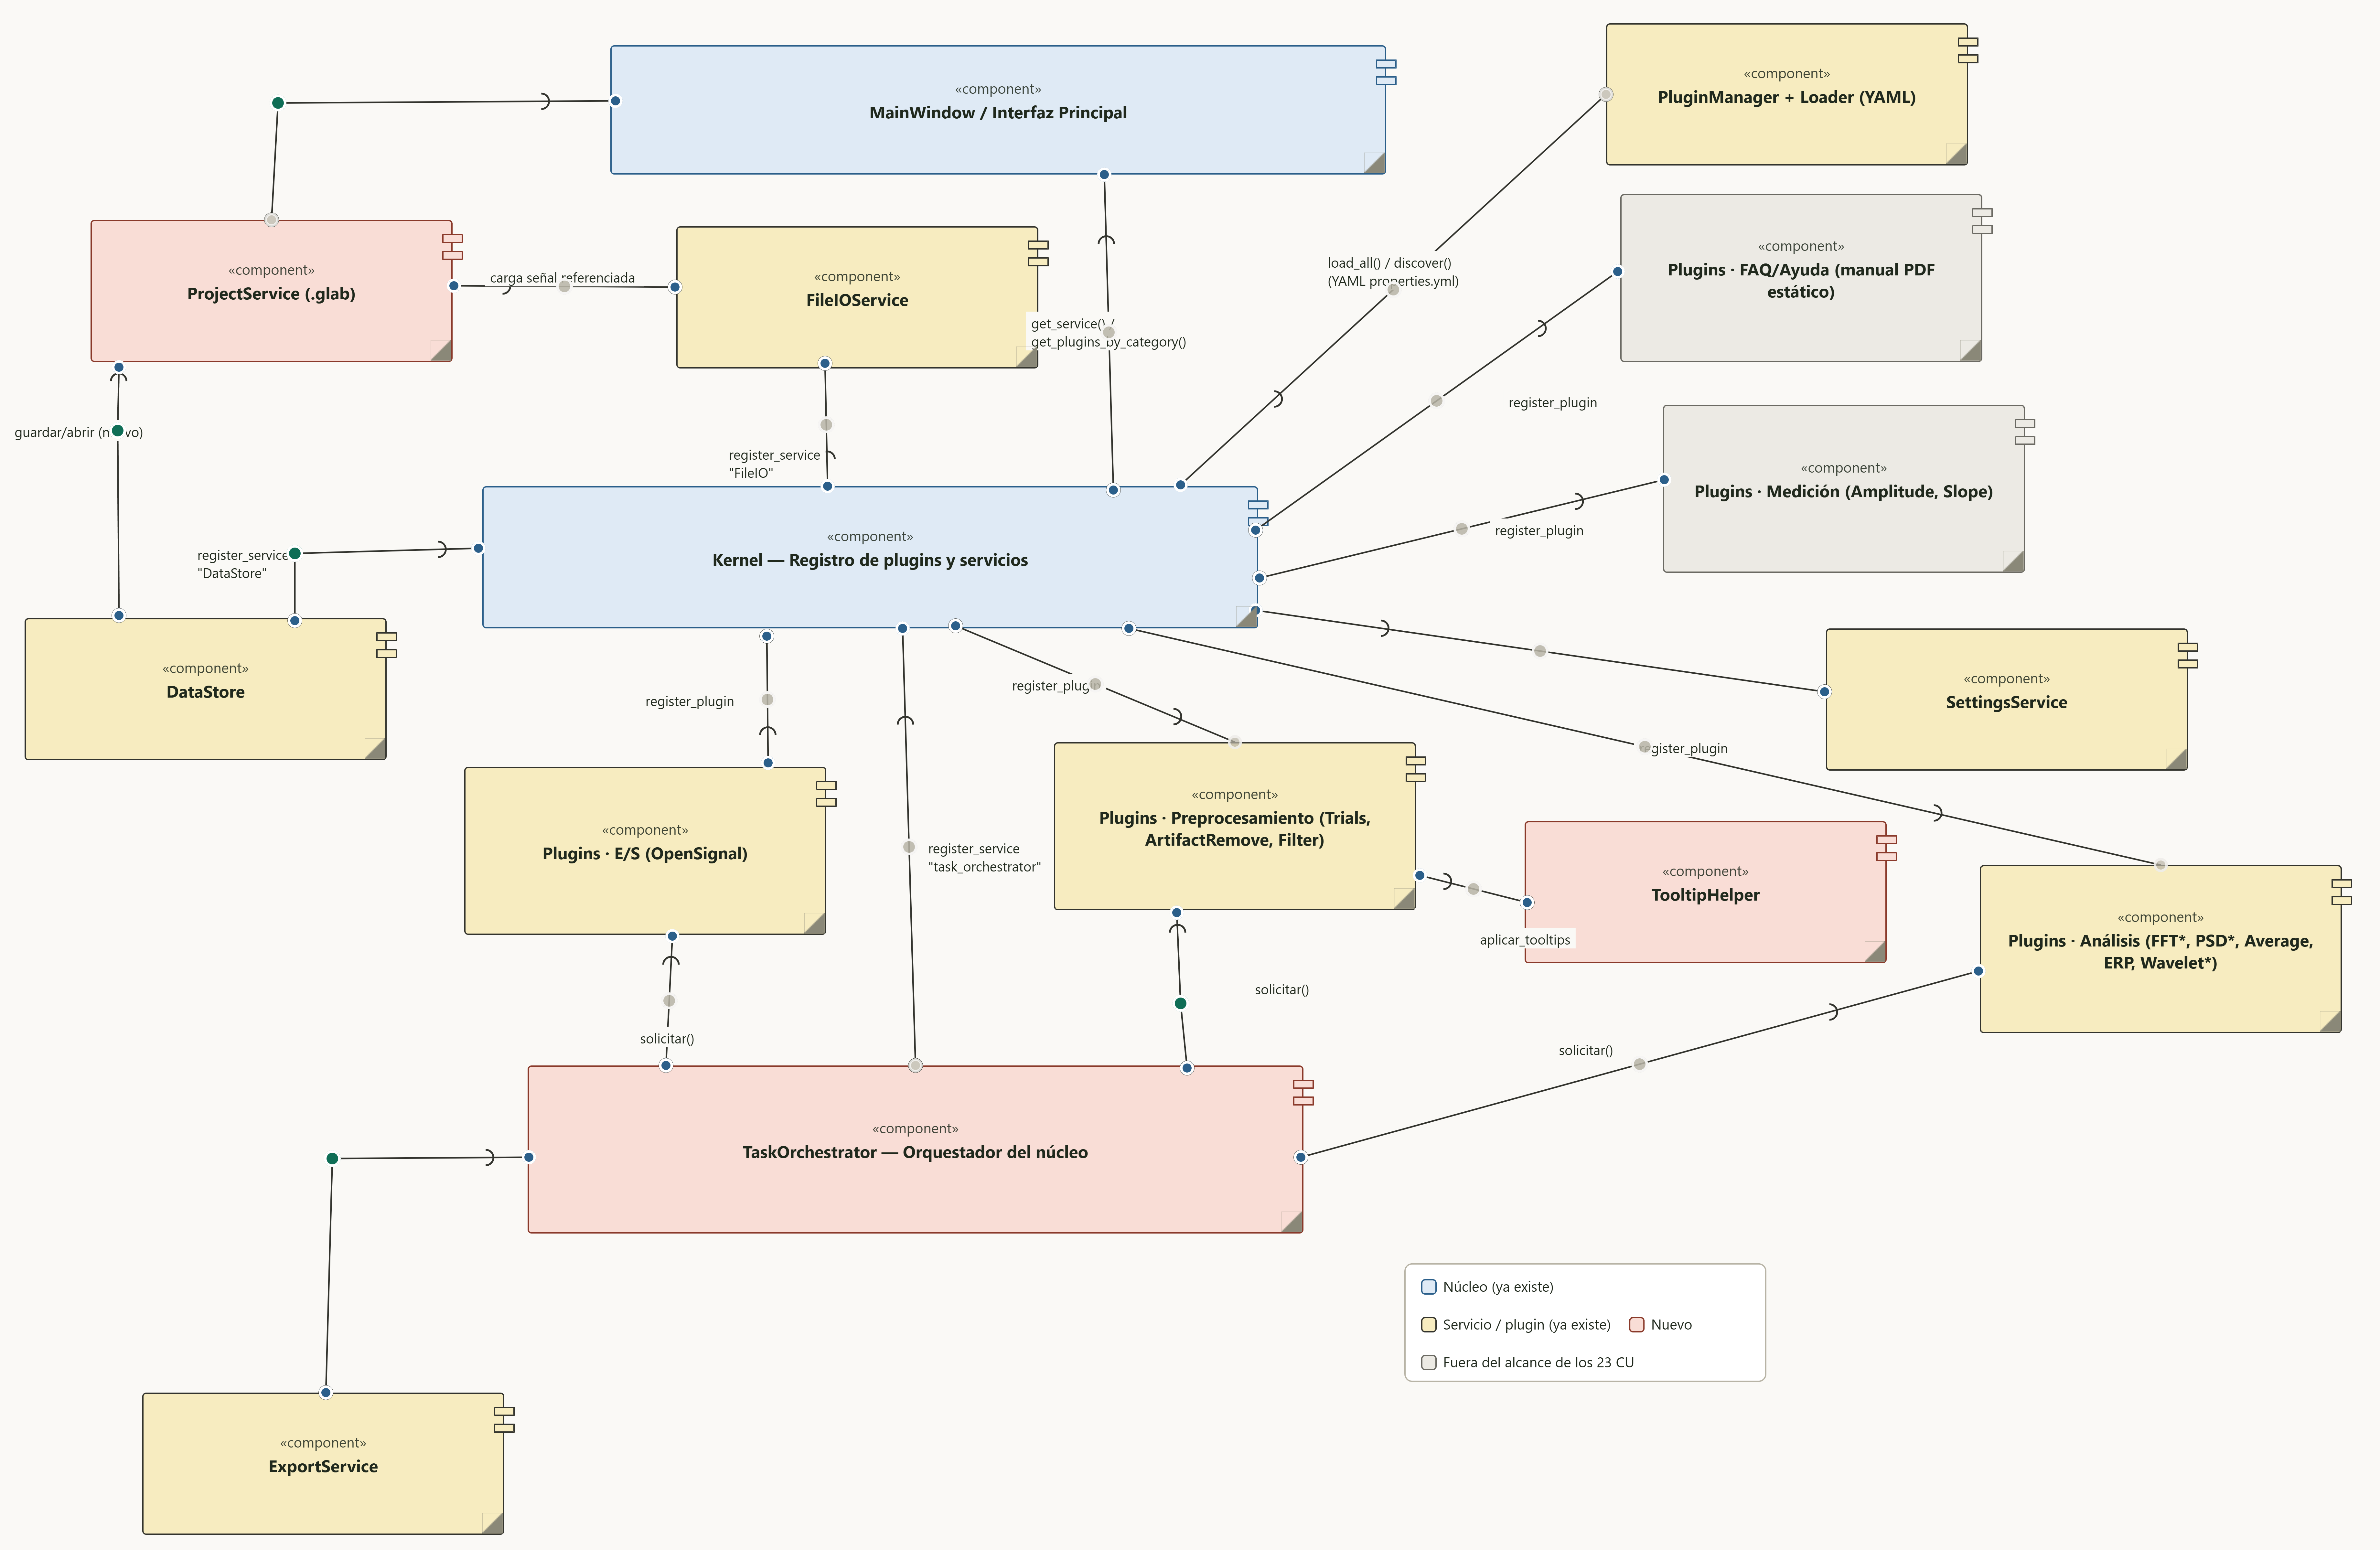
\includegraphics[width=0.95\linewidth]{diagrama_componentes_sistema_completo.png}
    \caption{Vista de desarrollo: componentes de Gamma Lab 2.0 agrupados por paquete real (\texttt{io}, \texttt{preprocessing}, \texttt{analysis}, \texttt{measure}, \texttt{faq}) m\'as los componentes nuevos transversales.}
    \label{fig:vistadesarrollo}
\end{figure}

Dos hallazgos relevantes para la planificaci\'on de la implementaci\'on:
\begin{itemize}[nosep]
    \item Los paquetes \texttt{measure/} (Amplitude, Slope) y \texttt{faq/} (manual PDF est\'atico) existen en el c\'odigo pero \textbf{ninguno} de los 23 casos de uso los cubre --- se muestran en gris neutro para delimitar la frontera del alcance actual.
    \item \texttt{TooltipHelper} depende de los plugins de preprocesamiento y an\'alisis por igual (CU-010): su ausencia hoy no es aislada, sino transversal a $\sim$15 plugins que carecen de \textit{tooltips}, salvo dos excepciones puntuales ya presentes en \texttt{TrialsPlugin} y \texttt{RelativePSDPlugin}.
\end{itemize}

\subsection{Vista de Procesos}
La vista de procesos describe el comportamiento din\'amico del sistema completo como un \'unico flujo maestro de sesi\'on, construido a partir de las cadenas de precondici\'on declaradas por las propias 23 fichas (p.\,ej. CU-006 exige trials generados por CU-004, que a su vez exige una se\~nal cargada por CU-003) --- no es una fusi\'on literal de los 23 flujos detallados, que ser\'ia ileg\'ible.

\begin{figure}[htbp]
    \centering
    \includegraphics[width=0.95\linewidth]{diagrama_actividad_sistema_completo.png}
    \caption{Flujo maestro de sesi\'on de Gamma Lab 2.0, con carriles Investigador/Sistema. Verde = ya existe, rojo = nuevo, blanco = mixto.}
    \label{fig:vistaprocesos}
\end{figure}

El flujo de la Figura \ref{fig:vistaprocesos} se organiza en las siguientes etapas:

\begin{enumerate}[nosep]
    \item \textbf{Inicio.} El sistema registra los servicios del n\'ucleo y descubre los plugins v\'ia YAML (CU-011); el registro del servicio de tareas en este paso es nuevo, el resto ya existe en \texttt{main.py}.
    \item \textbf{Apertura o carga.} Seg\'un si el investigador abre un \texttt{.glab} (CU-023, nuevo) o carga una se\~nal desde Home vac\'io (CU-003, ya existe v\'ia \texttt{FileIOService}), la se\~nal activa termina public\'andose en \texttt{DataStore}.
    \item \textbf{Preprocesamiento.} Generaci\'on/edici\'on de trials, selecci\'on de trials, remoci\'on de artefactos, filtrado y ajuste de frecuencia de muestreo (CU-004, CU-006, CU-007, CU-016, CU-018) --- los cuatro plugins ya existen en el c\'odigo.
    \item \textbf{An\'alisis.} PAC/PPC (CU-001, CU-002, nuevos), Wavelet (CU-013), promedio de trials (CU-015).
    \item \textbf{Orquestaci\'on.} Todo c\'omputo pesado se despacha al orquestador del n\'ucleo (CU-020, nuevo), cancelable en cualquier momento (CU-014, nuevo).
    \item \textbf{Visualizaci\'on.} Interacci\'on visual con el resultado, con submuestreo si la se\~nal es pesada (CU-012 parcial + CU-019, nuevo).
    \item \textbf{Iteraci\'on o cierre.} Si el investigador contin\'ua trabajando, el flujo retorna al preprocesamiento; de lo contrario, exporta y/o guarda el proyecto (CU-005 parcial, CU-017 nuevo) y cierra el proyecto y/o la aplicaci\'on (CU-021 nuevo, CU-022 parcial).
\end{enumerate}

A diferencia de Gamma Lab 1.0, los casos de uso de navegaci\'on (CU-008), limpieza de formulario (CU-009, 0\% implementado) y ayuda contextual (CU-010, cobertura parcial en solo 2 de m\'as de 15 plugins) son transversales a toda la sesi\'on: no ocupan un lugar fijo en la secuencia y se documentan como notas adjuntas al diagrama en lugar de forzarlas dentro del flujo principal.

\subsection{Vista F\'isica}
La vista f\'isica describe el entorno de despliegue local de Gamma Lab 2.0. A diferencia de Gamma Lab 1.0, aqu\'i se documenta expl\'icitamente la superficie completa de entrada/salida del sistema, incluyendo los artefactos que a\'un no existen.

\begin{figure}[htbp]
    \centering
    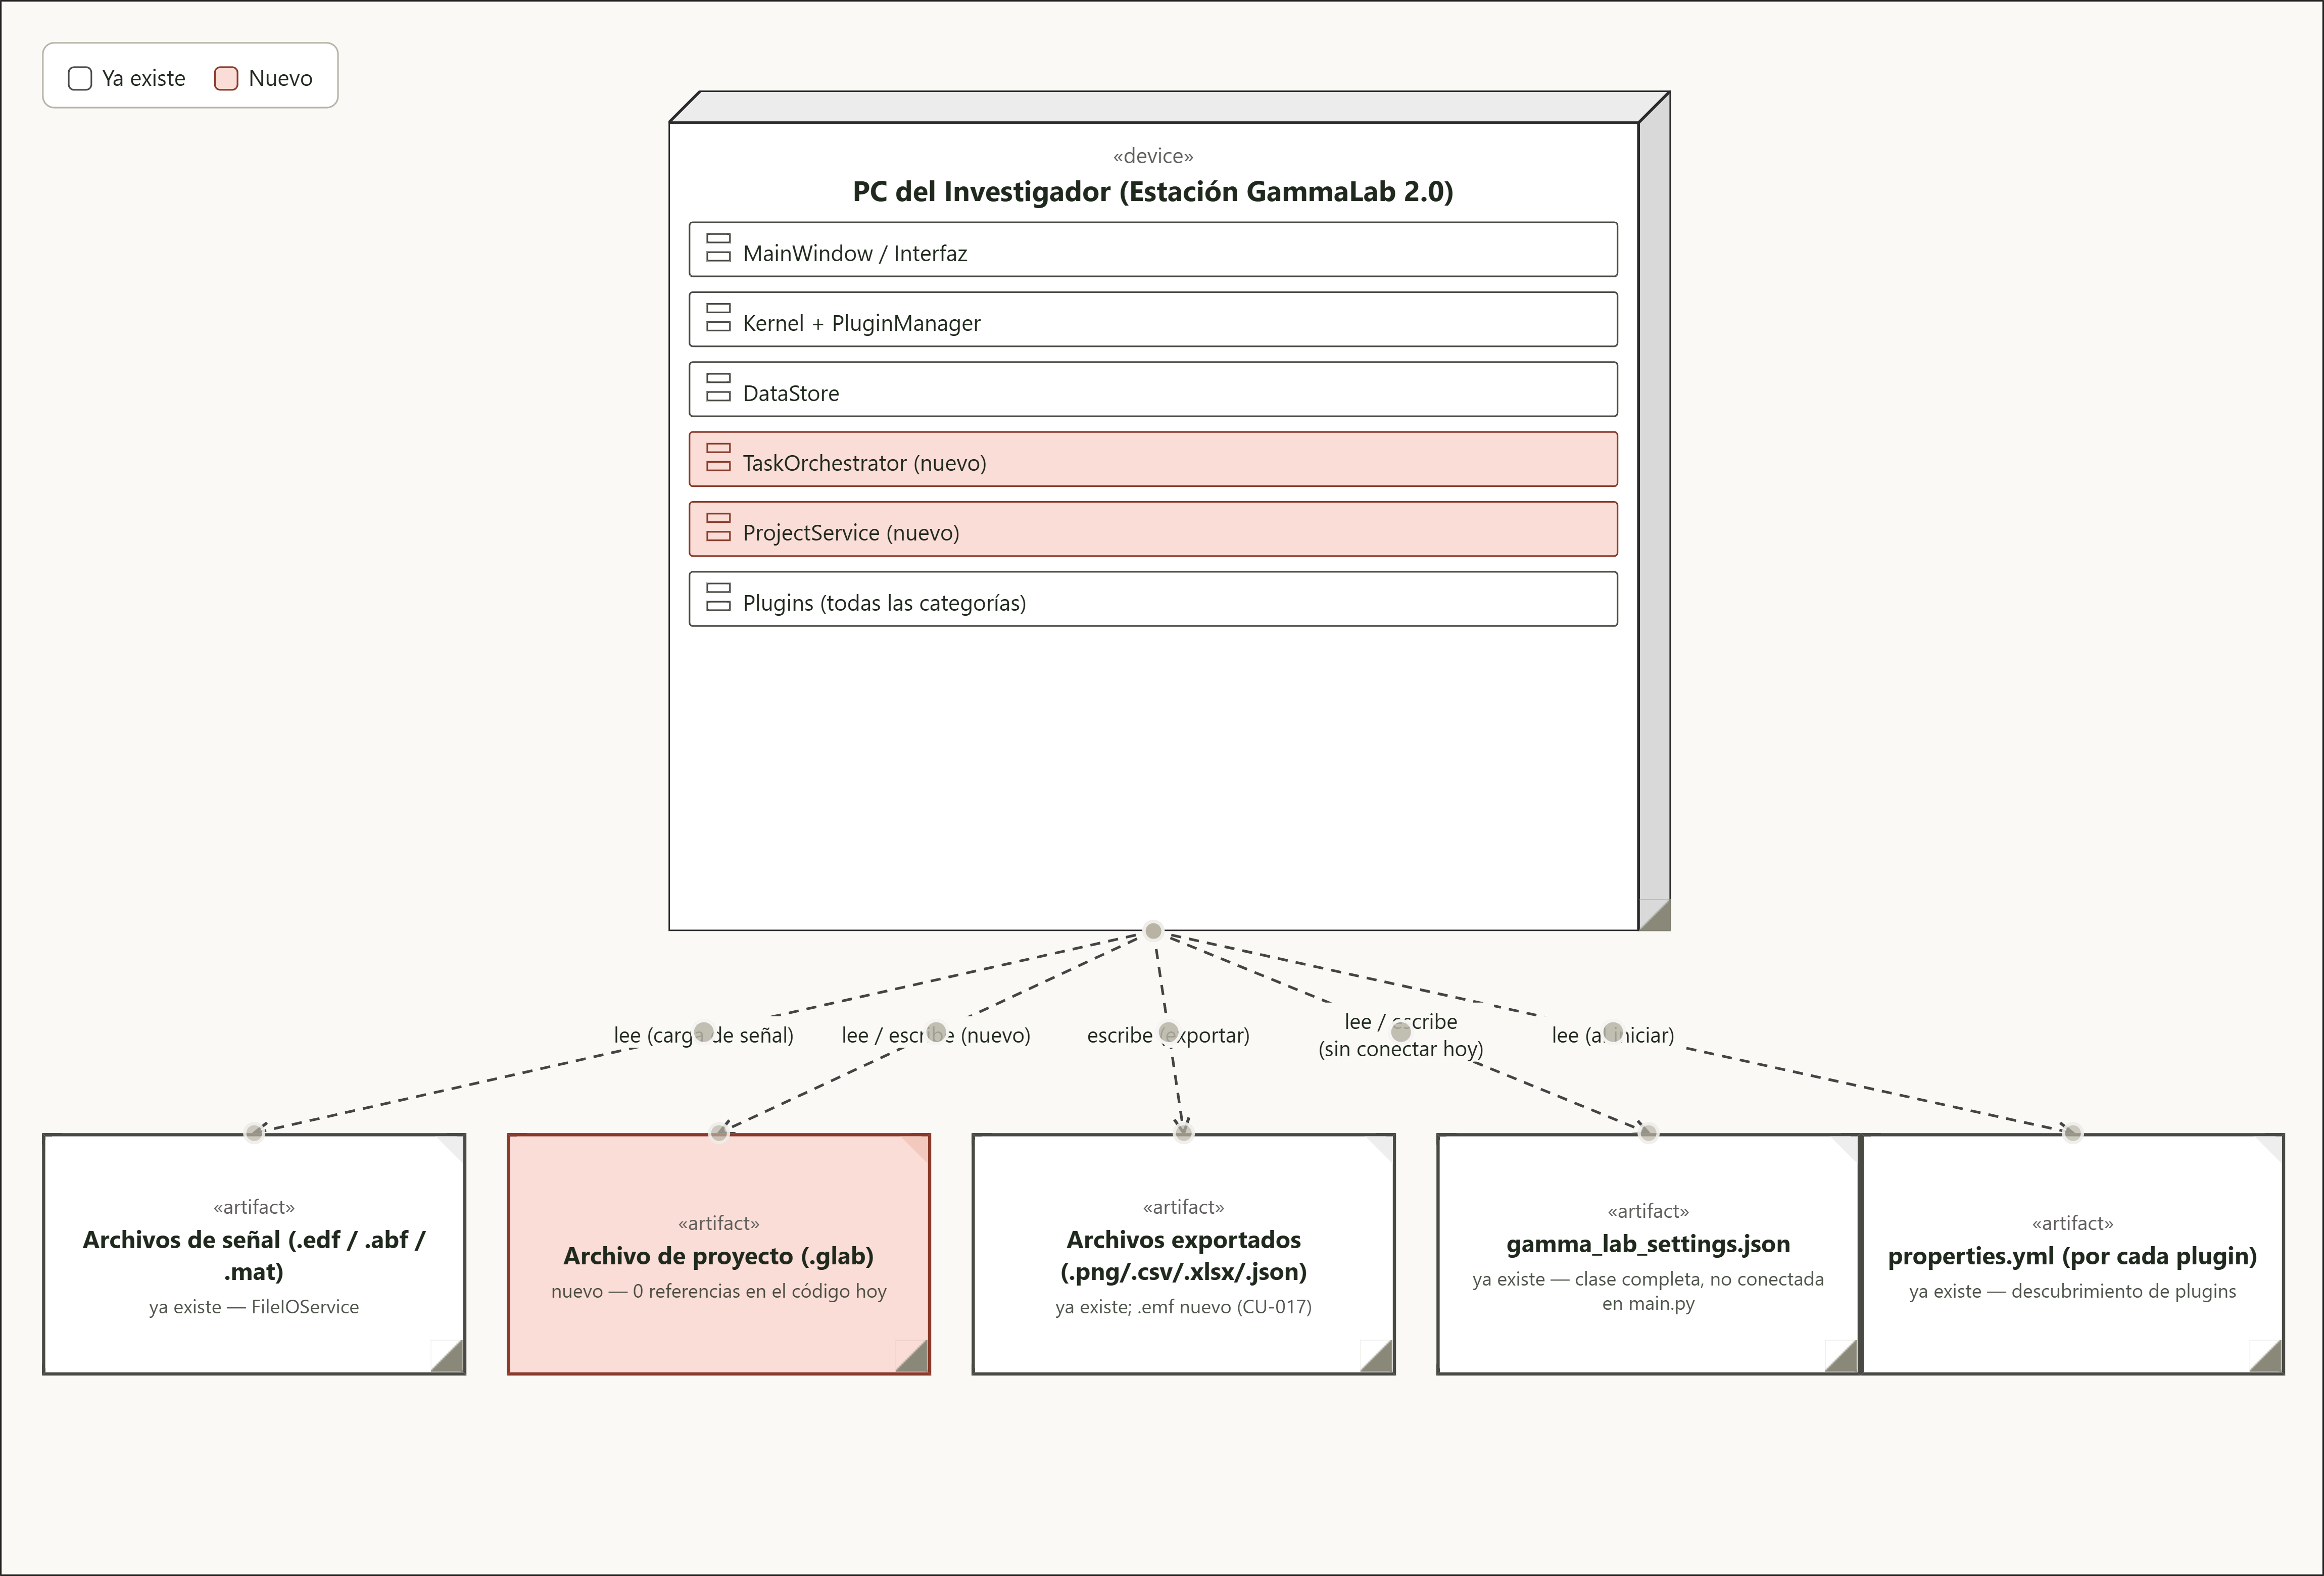
\includegraphics[width=0.85\linewidth]{diagrama_despliegue_sistema_completo.png}
    \caption{Vista f\'isica de Gamma Lab 2.0: estaci\'on \'unica de escritorio y su superficie de E/S.}
    \label{fig:vistafisica}
\end{figure}

La Figura \ref{fig:vistafisica} muestra el despliegue t\'ipico:
\begin{itemize}[nosep]
    \item Un \'unico nodo \textit{PC del Investigador}: no existe arquitectura cliente-servidor en ninguna de las 23 fichas.
    \item \textbf{Archivos de se\~nal} (\texttt{.edf}/\texttt{.abf}/\texttt{.mat}): ya existe, le\'idos por \texttt{FileIOService}.
    \item \textbf{Archivo de proyecto} (\texttt{.glab}): \textbf{nuevo} --- cero referencias en el c\'odigo actual.
    \item \textbf{Archivos exportados} (\texttt{.png}/\texttt{.csv}/\texttt{.xlsx}/\texttt{.json}): ya existe v\'ia \texttt{ExportService}; el formato vectorial \texttt{.emf} (CU-017) es nuevo.
    \item \texttt{gamma\_lab\_settings.json}: la clase \texttt{SettingsService} ya existe, pero \textbf{no} est\'a conectada en el arranque (\texttt{main.py}) hoy.
    \item \texttt{properties.yml} (por cada plugin): ya existe, sostiene el descubrimiento autom\'atico de plugins.
\end{itemize}



% ======================================================================
\section{Atributos de calidad}

\subsection{Escenarios de calidad}


\subsubsection{Escenario de Calidad 1: Integración de un Plugin Externo}

\begin{table}[H]
\centering
\caption{Escenario de calidad 1 --- Integración de un plugin externo}
\label{tab:escenario1}
\begin{tabularx}{\textwidth}{|l|X|}
\hline
\textbf{Aspecto} & \textbf{Descripción} \\
\hline
Atributo de calidad & Soporte \\
\hline
Requisito & El sistema debe permitir integrar plugins externos sin recompilar el núcleo y sin afectar módulos existentes. \\
\hline
Fuente del estímulo & Desarrollador externo \\
\hline
Estímulo & Se agrega un nuevo plugin a la carpeta de Plugins siguiendo el formato definido por el Kernel. \\
\hline
Artefacto & Módulo core del sistema (Kernel) y módulo de plugins. \\
\hline
Ambiente & Sistema en operación normal con múltiples plugins ya registrados. \\
\hline
Respuesta & El sistema detecta, valida y registra el plugin, exponiéndolo en la interfaz de usuario. \\
\hline
Medida de Respuesta & Plugin visible en la UI en menos de 1 minuto. Ningún plugin existente debe fallar tras la carga. \\
\hline
Trazabilidad & NFR-S-05 (R77--R78) \\
\hline
\end{tabularx}
\end{table}

\subsubsection{Escenario de Calidad 2: Carga de Señal de Gran Tamaño}

\begin{table}[H]
\centering
\caption{Escenario de calidad 2 --- Carga de señal de gran tamaño}
\label{tab:escenario2}
\begin{tabularx}{\textwidth}{|l|X|}
\hline
\textbf{Aspecto} & \textbf{Descripción} \\
\hline
Atributo de calidad & Rendimiento \\
\hline
Requisito & El sistema debe gestionar señales de gran tamaño sin bloqueos ni degradación significativa del rendimiento. \\
\hline
Fuente del estímulo & Usuario final \\
\hline
Estímulo & Se carga un archivo ABF/EDF de gran tamaño (ej. 1--2 GB, múltiples canales). \\
\hline
Artefacto & FileIOService, DatasetService (DataStore), servicio de tareas del núcleo, interfaz de usuario. \\
\hline
Ambiente & Computador con carga moderada y otros procesos del sistema activos. \\
\hline
Respuesta & La señal se carga correctamente, sin duplicación innecesaria de datos y sin bloqueos de la interfaz; la lectura corre en el servicio de tareas, fuera del hilo de la UI. \\
\hline
Medida de Respuesta & Visualización inicial en menos de 8 segundos para este caso de estrés (el umbral base de carga es $\leq 2$ s para el archivo típico de referencia). Uso de CPU menor a 80\%. Sin cierres inesperados ni latencias mayores a 5 segundos. \\
\hline
Trazabilidad & NFR-P-03 (R48), NFR-P-14 (R72), NFR-P-10 (R56) \\
\hline
\end{tabularx}
\end{table}

\subsubsection{Escenario de Calidad 3: Manejo de Errores en Tiempo de Ejecución}

\begin{table}[H]
\centering
\caption{Escenario de calidad 3 --- Manejo de errores en tiempo de ejecución}
\label{tab:escenario3}
\begin{tabularx}{\textwidth}{|l|X|}
\hline
\textbf{Aspecto} & \textbf{Descripción} \\
\hline
Atributo de calidad & Confiabilidad \\
\hline
Requisito & El sistema debe manejar excepciones en los plugins sin comprometer la estabilidad del sistema. \\
\hline
Fuente del estímulo & Sistema o entorno \\
\hline
Estímulo & Un plugin genera una excepción interna durante un análisis (FFT, PSD, Wavelet, ERP, PAC, etc.). \\
\hline
Artefacto & Módulo de plugins, Kernel, servicios asociados a cada plugin. \\
\hline
Ambiente & Análisis en curso con señales cargadas y otros plugins activos. \\
\hline
Respuesta & El sistema captura la excepción, informa al usuario y evita un cierre inesperado de la aplicación, manteniendo el Kernel operando de manera adecuada. \\
\hline
Medida de Respuesta & 0\% de pérdida de datos. Continuidad del sistema garantizada. Mensaje de error mostrado en menos de 2 segundos. \\
\hline
Trazabilidad & R47 \\
\hline
\end{tabularx}
\end{table}

\subsubsection{Escenario de Calidad 4: Exportación de Datos o Gráficas}

\begin{table}[H]
\centering
\caption{Escenario de calidad 4 --- Exportación de datos o gráficas}
\label{tab:escenario4}
\begin{tabularx}{\textwidth}{|l|X|}
\hline
\textbf{Aspecto} & \textbf{Descripción} \\
\hline
Atributo de calidad & Confiabilidad \\
\hline
Requisito & El sistema debe exportar gráficos y datos sin errores, incluso si se presentan fallas externas por disco, permisos, memoria u otros motivos. \\
\hline
Fuente del estímulo & Usuario final \\
\hline
Estímulo & El usuario exporta una tabla, medición o gráfico en PNG/CSV/JSON. \\
\hline
Artefacto & ExportService (registrado en el núcleo por inversión de control), interfaz de usuario, sistema de archivos. \\
\hline
Ambiente & Sistema operando con múltiples análisis realizados previamente sin guardar. \\
\hline
Respuesta & El archivo se genera correctamente o, en caso de error, se notifica al usuario sin afectar el estado del sistema. \\
\hline
Medida de Respuesta & Tiempo de exportación menor a 3 segundos. 0\% de pérdida de datos. Notificación clara ante error. \\
\hline
Trazabilidad & NFR-P-07 (R51), NFR-P-12 (R57), NFR-S-03 (R70) \\
\hline
\end{tabularx}
\end{table}

\subsubsection{Escenario de Calidad 5: Uso del Sistema sin Experiencia Técnica}

\begin{table}[H]
\centering
\caption{Escenario de calidad 5 --- Operación por un usuario sin experiencia técnica}
\label{tab:escenario5}
\begin{tabularx}{\textwidth}{|l|X|}
\hline
\textbf{Aspecto} & \textbf{Descripción} \\
\hline
Atributo de calidad & Usabilidad \\
\hline
Requisito & El sistema debe ser utilizable por un usuario con experiencia en neurociencias o análisis de señales, pero sin conocimientos profundos del software. \\
\hline
Fuente del estímulo & Usuario final \\
\hline
Estímulo & El usuario utiliza un plugin complejo como Wavelet, PSD o PAC por primera vez. \\
\hline
Artefacto & Interfaz de usuario, ayudas contextuales, parámetros preconfigurados. \\
\hline
Ambiente & Uso sin acompañamiento técnico. \\
\hline
Respuesta & El usuario puede completar el análisis apoyándose en la interfaz, con guía clara y sin errores operativos. \\
\hline
Medida de Respuesta & Análisis realizado en menos de 5 minutos. Bajo número de consultas al manual de usuario. \\
\hline
Trazabilidad & NFR-U-07 (R42), NFR-U-08 (R43), NFR-U-05 (R10), NFR-U-09 (R44) \\
\hline
\end{tabularx}
\end{table}

\subsubsection{Escenario de Calidad 6: Rendimiento con Múltiples Señales Cargadas}

\begin{table}[H]
\centering
\caption{Escenario de calidad 6 --- Rendimiento con múltiples señales cargadas}
\label{tab:escenario6}
\begin{tabularx}{\textwidth}{|l|X|}
\hline
\textbf{Aspecto} & \textbf{Descripción} \\
\hline
Atributo de calidad & Rendimiento \\
\hline
Requisito & El sistema debe mantener tiempos de respuesta estables aun cuando varias señales se encuentren cargadas simultáneamente dentro de la misma ProjectSession. \\
\hline
Fuente del estímulo & Usuario final \\
\hline
Estímulo & El usuario carga entre 2 y 4 señales de gran tamaño y ejecuta diferentes análisis en cada una. \\
\hline
Artefacto & DataStore, gestor de vistas, motor de análisis. \\
\hline
Ambiente & Sistema operando con alto volumen de datos en memoria. \\
\hline
Respuesta & El sistema reutiliza datos sin duplicarlos, mantiene tiempos de acceso aceptables y evita bloqueos en la interfaz. \\
\hline
Medida de Respuesta & Cambio entre señales cargadas en menos de 1 segundo. Sin bloqueos ni cierres inesperados. Uso de memoria dentro del 70--75\%. \\
\hline
Trazabilidad & NFR-P-06 (R51), NFR-P-01/P-08 (R11, R53) \\
\hline
\end{tabularx}
\end{table}

\subsubsection{Escenario de Calidad 7: Resiliencia ante Archivos Corruptos o Incompatibles}

\begin{table}[H]
\centering
\caption{Escenario de calidad 7 --- Resiliencia ante archivos corruptos o incompatibles}
\label{tab:escenario7}
\begin{tabularx}{\textwidth}{|l|X|}
\hline
\textbf{Aspecto} & \textbf{Descripción} \\
\hline
Atributo de calidad & Confiabilidad \\
\hline
Requisito & El sistema debe detectar archivos corruptos, incompletos o incompatibles sin comprometer la estabilidad del programa. \\
\hline
Fuente del estímulo & Usuario final o sistema externo \\
\hline
Estímulo & El usuario intenta cargar un archivo ABF/EDF/MAT con estructura inválida o con metadatos corruptos. \\
\hline
Artefacto & FileIOService, Kernel, sistema de alertas. \\
\hline
Ambiente & Sistema en operación normal con señales previamente cargadas. \\
\hline
Respuesta & El sistema captura el error, notifica al usuario, cancela la operación de carga y mantiene intacta la sesión actual. \\
\hline
Medida de Respuesta & Mensaje de error mostrado en menos de 2 segundos. 0\% de pérdida de datos o señales cargadas previamente. El sistema continúa operativo sin fallos. \\
\hline
Trazabilidad & FR-IO-04  \\
\hline
\end{tabularx}
\end{table}

\subsubsection{Escenario de Calidad 8: Consistencia entre Datos Ingresados y Gráficas Generadas}

\begin{table}[H]
\centering
\caption{Escenario de calidad 8 --- Consistencia entre datos ingresados y gráficas generadas}
\label{tab:escenario8}
\begin{tabularx}{\textwidth}{|l|X|}
\hline
\textbf{Aspecto} & \textbf{Descripción} \\
\hline
Atributo de calidad & Confiabilidad y Usabilidad \\
\hline
Requisito & El sistema debe garantizar que las gráficas generadas correspondan fielmente a los datos y parámetros seleccionados por el usuario. \\
\hline
Fuente del estímulo & Usuario final \\
\hline
Estímulo & El usuario modifica parámetros como canal, ventana temporal, trials seleccionados o rango de frecuencias. \\
\hline
Artefacto & Interfaz de usuario, motor de visualización, servicios de análisis. \\
\hline
Ambiente & Sistema ejecutando análisis consecutivos sobre diferentes configuraciones. \\
\hline
Respuesta & La gráfica generada refleja exactamente los datos filtrados o seleccionados, sin desajustes ni inconsistencias con los parámetros ingresados. \\
\hline
Medida de Respuesta & Actualización gráfica en menos de 3 segundos. 0 diferencias entre los datos mostrados y los procesados. Consistencia confirmada entre ejecuciones sucesivas. \\
\hline
Trazabilidad & NFR-R-04 (R73), NFR-U-02 (R03) \\
\hline
\end{tabularx}
\end{table}




\subsection{Reglas de compatibilidad y versionado}

\begin{itemize}
    \item \textbf{Versionado de la aplicaci\'on.} GammaLab 2.0 adopta versionado sem\'antico \texttt{MAJOR.\allowbreak MINOR.\allowbreak PATCH}: \texttt{MAJOR} rompe \texttt{.glab} o el contrato \texttt{IPlugin}; \texttt{MINOR} agrega capacidades retrocompatibles; \texttt{PATCH} corrige sin alterar contratos p\'ublicos. \texttt{main.py} expone esta versi\'on en una constante \'unica, visible en un di\'alogo ``Acerca de'' y embebida como metadato en cada archivo \texttt{.glab} generado.

    \item \textbf{Contrato de plugins (\texttt{IPlugin}).} Cambios aditivos (nuevos m\'etodos opcionales, nuevos campos con valor por defecto) no rompen compatibilidad. Cambios que alteren la firma de \texttt{initialize}, \texttt{start}, \texttt{stop}, \texttt{process} o \texttt{get\_widget} elevan la versi\'on \texttt{MAJOR} del contrato.

    \item \textbf{Metadatos \texttt{properties.yml}.} Los campos requeridos (\texttt{id, name, category, subcategory, version, icon, logic\_class, ui\_class}) deben existir siempre -- exigido por \texttt{REQUIRED\_\allowbreak KEYS} en \texttt{loader.py} -- y a\~nadir campos opcionales es compatible. El campo \texttt{version} declara el \texttt{MAJOR} de \texttt{IPlugin} contra el que se escribi\'o el plugin; \texttt{discover()} rechaza el plugin si no coincide con el \texttt{MAJOR} del n\'ucleo en ejecuci\'on.

    \item \textbf{Formato de proyecto \texttt{.glab}.} \texttt{ProjectService} persiste el espacio de trabajo -- se\~nal activa, trials y an\'alisis -- en archivos \texttt{.glab}. Cada \texttt{.glab} embebe un \texttt{schema\_version} propio: un incremento \texttt{MINOR} se mantiene legible por versiones futuras de \texttt{ProjectService}, y un incremento \texttt{MAJOR} rechaza la apertura con un mensaje expl\'icito al usuario en vez de migrar impl\'icitamente.

    \item \textbf{Dependencias externas.} \texttt{requirements.txt} fija cada librer\'ia con versi\'on exacta (\texttt{==}), sin rangos abiertos (Tabla~\ref{tab:deps}). Actualizar VTK, SciPy, PyWavelets o NumPy exige re-ejecutar completas las suites \texttt{plugins\_\allowbreak test} y \texttt{performance\_\allowbreak test} antes de aceptar el cambio.

    \item \textbf{Formatos de se\~nal externos (EDF/ABF/BDF/MAT).} La compatibilidad se ancla a la versi\'on de la librer\'ia lectora (\texttt{pyabf}, \texttt{pyedflib}), no al formato en s\'i. Un archivo no interpretable por esa versi\'on se reporta como incompatible, sin remuestreo ni heur\'isticas de recuperaci\'on impl\'icitas: un EDF con canales a distinta frecuencia de muestreo falla con un mensaje claro, en vez de intentar corregirse autom\'aticamente.

    \item \textbf{Estabilidad de m\'odulos internos.} Todo renombramiento o reubicaci\'on de un m\'odulo p\'ublico de \texttt{core/} actualiza en el mismo cambio a todos sus consumidores, tests incluidos, y un flujo de CI corre \texttt{pytest} en cada \textit{push}/\textit{pull request}. Motivo: un renombramiento previo de \texttt{fileio.py} a \texttt{fileio\_\allowbreak service.py} (con \texttt{TrialDataset} movido a \texttt{core/\allowbreak model/}) rompi\'o silenciosamente los 8 archivos de \texttt{plugins\_\allowbreak test} al no actualizarse en el mismo cambio.
\end{itemize}

\begin{center}
\small
\begin{longtable}{|p{0.30\textwidth}|p{0.20\textwidth}|p{0.30\textwidth}|}
\caption{Versiones de dependencias externas ancladas en \texttt{requirements.txt}} \label{tab:deps} \\
\hline
\textbf{Librer\'ia} & \textbf{Versi\'on} & \textbf{Rol} \\
\hline
\endfirsthead
\hline
\textbf{Librer\'ia} & \textbf{Versi\'on} & \textbf{Rol} \\
\hline
\endhead
\texttt{numpy} & 2.3.4 & C\'alculo num\'erico vectorizado \\
\hline
\texttt{scipy} & 1.16.2 & Filtros, PSD (Welch) \\
\hline
\texttt{PyWavelets} & 1.9.0 & Transformada Wavelet Continua \\
\hline
\texttt{vtk} & 9.5.2 & Renderizado cient\'ifico 2D/3D \\
\hline
\texttt{PyQt5} / \texttt{PyQt5-Qt5} & 5.15.11 / 5.15.2 & Interfaz gr\'afica \\
\hline
\texttt{pyabf} & 2.3.8 & Lectura de archivos \texttt{.abf} \\
\hline
\texttt{pyEDFlib} & 0.1.42 & Lectura de archivos \texttt{.edf} \\
\hline
\texttt{h5py} & 3.15.1 & Soporte de formatos basados en HDF5 \\
\hline
\texttt{pytest} & 8.4.2 & Framework de pruebas \\
\hline
\end{longtable}
\end{center}

\subsection{M\'etricas y plan de verificaci\'on}

La Tabla~\ref{tab:metricas} formaliza la ``Medida de Respuesta'' de cada escenario de calidad (secci\'on~5.1) en una m\'etrica verificable, junto con su m\'etodo de medici\'on y el criterio de aceptaci\'on correspondiente.

\begin{center}
\small
\begin{longtable}{|p{0.16\textwidth}|p{0.19\textwidth}|p{0.21\textwidth}|p{0.28\textwidth}|}
\caption{M\'etricas, m\'etodo de verificaci\'on y criterio de aceptaci\'on por atributo de calidad} \label{tab:metricas} \\
\hline
\textbf{Atributo} & \textbf{M\'etrica} & \textbf{M\'etodo} & \textbf{Criterio de aceptaci\'on} \\
\hline
\endfirsthead
\hline
\textbf{Atributo} & \textbf{M\'etrica} & \textbf{M\'etodo} & \textbf{Criterio de aceptaci\'on} \\
\hline
\endhead
\hline
\multicolumn{4}{r}{\textit{Contin\'ua en la siguiente p\'agina}} \\
\endfoot
\hline
\endlastfoot

Extensibilidad (Esc.~1) &
Tiempo de aparici\'on de un plugin nuevo; plugins existentes que fallan &
Agregar un plugin v\'alido y correr \texttt{plugins\_\allowbreak test} &
$<$1\,min; 0 plugins fallan (R77--R78) \\
\hline

Rendimiento -- carga grande (Esc.~2) &
Tiempo a primer render; uso de CPU &
\texttt{performance\_\allowbreak test}; medido: 78.4\,ms (1.8\,M muestras) &
$\leq$8\,s estr\'es, $\leq$2\,s t\'ipico; CPU $<$80\% (R48/R72/R56) \\
\hline

Confiabilidad -- errores en ejecuci\'on (Esc.~3) &
\% p\'erdida de datos; tiempo del mensaje &
Inyecci\'on de fallos dentro de \texttt{process()} &
0\% p\'erdida; mensaje $<$2\,s; sistema operativo \\
\hline

Confiabilidad -- exportaci\'on (Esc.~4) &
Tiempo de exportaci\'on; error silencioso &
\texttt{test\_\allowbreak export.py} &
$<$3\,s; 0\% p\'erdida; notificaci\'on clara (R51/R57/R70) \\
\hline

Usabilidad (Esc.~5) &
Tiempo de an\'alisis sin acompa\~namiento &
Prueba de usabilidad con usuarios reales &
$<$5\,min; bajas consultas al manual (R42--R44) \\
\hline

Rendimiento -- m\'ultiples se\~nales (Esc.~6) &
Tiempo de cambio; \% de memoria &
Benchmark de \texttt{DataStore} &
$<$1\,s cambio; memoria 70--75\% (R11, R51, R53) \\
\hline

Confiabilidad -- archivos corruptos (Esc.~7) &
Tiempo del error; continuidad de sesi\'on &
\texttt{test\_\allowbreak fileio\_\allowbreak abf}/\texttt{edf.py} &
Mensaje $<$2\,s; 0\% p\'erdida previa (FR-IO-04) \\
\hline

Confiabilidad y\newline Usabilidad (Esc.~8) &
Tiempo de actualizaci\'on; diferencias &
Revisi\'on de consistencia entrada-salida &
$<$3\,s; 0 diferencias (R73, R03) \\
\hline

Mantenibilidad &
\% de cobertura autom\'atica &
\texttt{pytest} --\texttt{cov} sobre \texttt{core}/\texttt{plugins} &
$\geq$80\% de cobertura \\
\hline

Rendimiento -- no regresi\'on vs.\ 1.0 &
Factor vs.\ l\'inea base &
\texttt{compare\_\allowbreak report.py} &
Nada empeora; render sin vectorizar mejora $\geq$10$\times$ \\
\hline

Portabilidad &
\'Exito de arranque del \texttt{.exe} &
Instalaci\'on en Windows limpio sin Python &
Arranque exitoso, sin configuraci\'on manual \\
\hline

Robustez --\newline cancelaci\'on (UC-02) &
Liberaci\'on del hilo tras cancelar &
Prueba forzada sobre \texttt{Task\-Orchestrator} &
Liberaci\'on garantizada (R46, R70, R74) \\
\hline

\end{longtable}
\end{center}

\subsection{Plan de evidencia}
\begin{enumerate}
    \item \textbf{Fixture ABF real y referencias MATLAB.} \texttt{test/data/17308005.abf} m\'as los 8 CSV de referencia en \texttt{plugins\_\allowbreak test/} sustentan la correcci\'on num\'erica exigida por Extensibilidad (Esc.~1) y por las m\'etricas de Mantenibilidad.
    \item \textbf{Suite de benchmarks versionada.} \texttt{performance\_\allowbreak test/}, con resultados persistidos por etiqueta en \texttt{perf\_\allowbreak results.json} (p.\,ej.\ \texttt{gammalab1\_\allowbreak baseline\_\allowbreak 2026-08-16}), es la evidencia reproducible de Rendimiento y de la comparaci\'on de no regresi\'on frente a 1.0.
    \item \textbf{Auditor\'ias documentales.} Los informes \texttt{reporte\_\allowbreak tests.\allowbreak tex} e \texttt{informe\_\allowbreak rendimiento.\allowbreak tex} (\texttt{docs/\allowbreak tests documents/}) registran el estado de la suite de pruebas y los hallazgos de rendimiento.
    \item \textbf{Pruebas de usabilidad con usuarios reales.} \texttt{docs/pruebas-usabilidad/} sustenta el criterio de aceptaci\'on de Usabilidad (Esc.~5).
    \item \textbf{Prueba de instalaci\'on limpia.} Arranque del ejecutable generado por PyInstaller en un Windows~10/11 sin Python previamente instalado, como evidencia de Portabilidad.
    \item \textbf{Registro de cancelaci\'on forzada.} La prueba de cancelaci\'on forzada sobre el \texttt{Task\-Orchestrator} bajo carga es la evidencia de Robustez (UC-02).
\end{enumerate}

\subsection{Conclusi\'on}

Los escenarios de calidad, las reglas de compatibilidad y la tabla de m\'etricas convierten los atributos de calidad de la secci\'on~3.2 en criterios operativos y verificables, no en aspiraciones gen\'ericas. El plan de evidencia de la secci\'on~6.4 sostiene estos criterios con artefactos reproducibles: fixtures reales validados contra una referencia de MATLAB, benchmarks versionados por etiqueta, auditor\'ias documentales, y pruebas de usabilidad y de instalaci\'on. Junto con las reglas de versionado de la secci\'on~6.2, esta estructura garantiza que la arquitectura de GammaLab~2.0 eval\'ue, documente y demuestre sus atributos de calidad de forma reproducible en cada nueva versi\'on del sistema.


% ======================================================================
\section{Anexos}



\subsection{Anexo A --- Relaci\'on con el SRS}


En particular:
\begin{itemize}
    \item 
\end{itemize}



\subsection{Anexo B --- Relaci\'on con el SDD}


Este anexo resume dicha relaci\'on:
\begin{itemize}
    \item 
\end{itemize}



\subsection{Anexo C --- Trazabilidad global de artefactos}


\subsection{Anexo D --- Diagramas y tablas de referencia}


% ======================================================================
\section{Referencias}

\begin{thebibliography}{99}

\bibitem{python} Python Software Foundation. \textit{Python 3 --- The Python Standard Library}. Disponible en: \url{https://docs.python.org/3/}.

\bibitem{pyqt5} Riverbank Computing. \textit{PyQt5 Reference Guide}. Disponible en: \url{https://www.riverbankcomputing.com/static/Docs/PyQt5/}.

\bibitem{qt5} The Qt Company. \textit{Qt 5 --- Style Sheets Reference}. Disponible en: \url{https://doc.qt.io/qt-5/stylesheet-syntax.html}.

\bibitem{vtk} Kitware, Inc. \textit{VTK --- Visualization Toolkit Documentation}. Disponible en: \url{https://vtk.org/} y \url{https://docs.vtk.org/}.

\bibitem{vtkchartxy} Kitware, Inc. \textit{vtkChartXY Class Reference}. Disponible en: \url{https://docs.vtk.org/en/latest/api/python/vtkmodules.vtkChartsCore.html\#vtkmodules.vtkChartsCore.vtkChartXY}.

\bibitem{numpy} NumPy Developers. \textit{NumPy Documentation}. Disponible en: \url{https://numpy.org/doc/}.

\bibitem{pyabf} Scott W. Harden. \textit{pyABF --- Read and Analyze ABF Files with Python}. Disponible en: \url{https://pyabf.readthedocs.io/}.

\bibitem{pyedflib} Holger Nahrstaedt et al. \textit{pyEDFlib --- Python library to read/write EDF+/BDF+ files}. Disponible en: \url{https://pyedflib.readthedocs.io/}.

\bibitem{yaml} Oren Ben-Kiki, Clark Evans, Ingy d\"ot Net. \textit{YAML Ain't Markup Language (YAML) Specification}. Disponible en: \url{https://yaml.org/spec/}.

\bibitem{kruchten} P. B. Kruchten. \textit{The 4+1 View Model of Architecture}. IEEE Software, vol. 12, no. 6, pp. 42--50, 1995. DOI: \url{https://doi.org/10.1109/52.469759}.

\bibitem{bass} Len Bass, Paul Clements, Rick Kazman. \textit{Software Architecture in Practice} (3rd ed.). Addison--Wesley, 2012. ISBN 978-0-321-81573-6.

\bibitem{clements} Paul Clements, Felix Bachmann, Len Bass, David Garlan, James Ivers, Reed Little, Robert Nord, Judith Stafford. \textit{Documenting Software Architectures: Views and Beyond} (2nd ed.). Addison--Wesley, 2010. ISBN 978-0-321-55268-6.

\bibitem{atam} Rick Kazman, Mark Klein, Paul Clements. \textit{ATAM: Method for Architecture Evaluation}. CMU/SEI-2000-TR-004, Software Engineering Institute, 2000.

\bibitem{edf} Bob Kemp, Alpo V\"arri, Agostinho Rosa, Kim D. Nielsen, John Gade. \textit{A simple format for exchange of digitized polygraphic recordings}. Electroencephalography and Clinical Neurophysiology, 82(5), 1992, pp. 391--393. DOI: \url{https://doi.org/10.1016/0013-4694(92)90009-7}.

\bibitem{nunez} P. L. Nunez, R. Srinivasan. \textit{Electric Fields of the Brain: The Neurophysics of EEG} (2nd ed.). Oxford University Press, 2006.

\bibitem{sad} Equipo Gamma Lab. \textit{Software Architecture Document (SAD), v1.0}. Este documento.

\end{thebibliography}

\vspace{0.5cm}
\noindent\textit{Nota}: Las URLs se\~naladas se incluyen para consulta r\'apida. En publicaci\'on impresa, usar DOI/ISBN cuando aplique.

\end{document}